\documentclass[12pt]{article}

\usepackage[latin1]{inputenc} 
\usepackage{amssymb} 
%\usepackage{lscape} 
\usepackage{amsmath}
\usepackage{amsthm}
\usepackage{mathtools}
%\usepackage{kmath}
\usepackage{txfonts}
\usepackage{latexsym}
\usepackage{subfigure}
\usepackage{graphicx}
\usepackage{bm}
\usepackage{bbm}
\usepackage{overpic}
\usepackage[normalem]{ulem}
\usepackage{url}
\usepackage{soul}
\usepackage{exscale}
\usepackage{amsfonts}
\usepackage[usenames,dvipsnames]{xcolor} % load color package
\usepackage{hyperref}
\usepackage{verbatim}
\usepackage[usenames,dvipsnames]{xcolor}
\usepackage{comment}
\usepackage{epsfig}

\textwidth=6.0in \textheight=8.8in \hoffset=-0.2in
\voffset=-0.85in
\parskip=6pt
%\lineskip=18pt
 \baselineskip=9pt
 \topmargin 0.8in
 
\def\black#1{\textcolor{black}{#1}}
\def\blue#1{\textcolor{blue}{#1}}
\def \red#1{\textcolor{red}{#1}}
\def\green#1{\textcolor{BlueGreen}{#1}}
\def\yellow#1{\textcolor{yellow}{#1}}
\def\orange{\textcolor{BurntOrange}}

%\numberwithin{equation}{section}

\newtheorem{definition}{Definition}[section]
\newtheorem{lemma}{Lemma}[section]
\newtheorem{remark}{Remark}[section]
\newtheorem{example}{Example}[section]
\newtheorem{theorem}{Theorem}[section]
\newtheorem{cor}{Corollary}[section]
\newtheorem{conj}{Conjecture}[section]
\newtheorem{prop}{Proposition}[section]


\numberwithin{equation}{section}
\numberwithin{figure}{section}


\newcommand{\E}{\mathbb{E}}
\newcommand{\R}{\mathbb{R}}
\newcommand{\sigl}{\sigma_L}
\newcommand{\BS}{\rm BS}
\newcommand{\p}{\partial}
\newcommand{\var}{{\rm var}}
\newcommand{\cov}{{\rm cov}}
\newcommand{\beas}{\begin{eqnarray*}}
\newcommand{\eeas}{\end{eqnarray*}}
\newcommand{\bea}{\begin{eqnarray}}
\newcommand{\eea}{\end{eqnarray}}
\newcommand{\ben}{\begin{enumerate}}
\newcommand{\een}{\end{enumerate}}

\newcommand{\wh}{\widehat}
\newcommand{\Ind}[1]{\mathbbm{1}_{\left\{#1\right\}}}
\newcommand{\Rplus}{\mathbb{R}_{\geqslant 0}}
\newcommand{\Rpplus}{\mathbb{R}_{> 0}}
\newcommand{\Rminus}{\mathbb{R}_{\leqslant 0}}
\newcommand{\wt}[1]{{\widetilde{#1}}}

\newcommand{\ui}{\mathrm{i}}
\newcommand{\mt}{\mathbf{t}}
\newcommand{\dm}{\diamond}
\newcommand{\sq}{\square}

%\newcommand{ \vardiamondsuit}
\newcommand{\mS}{\mathbf{S}}
\newcommand{\mA}{\mathbbm{A}}
\newcommand{\tC}{\widetilde{C}}
\newcommand{\hC}{\widehat{C}}
\newcommand{\tH}{\widetilde{H}}
\newcommand{\cD}{\mathcal{D}}
\newcommand{\cS}{\mathcal{S}}
\newcommand{\cR}{\mathcal{R}}
\newcommand{\cU}{\mathcal{U}}
\newcommand{\cL}{\mathcal{L}}
\newcommand{\cF}{\mathcal{F}}
\newcommand{\mF}{\mathbb{F}}
\newcommand{\mT}{\mathbb{T}}
\newcommand{\mK}{\mathbb{K}}
\newcommand{\Y}{Y}

\newcommand{\cV}{\mathcal{V}}
\newcommand{\cG}{\mathcal{G}}
\newcommand{\cv}{\mathcal{v}}
\newcommand{\cg}{\mathcal{g}}
\newcommand{\cH}{\mathcal{H}}
\newcommand{\cI}{\mathcal{I}}
\newcommand{\cK}{\mathcal{K}}
\newcommand{\cJ}{\mathcal{J}}
\newcommand{\cC}{\mathcal{C}}
\newcommand{\cE}{\mathcal{E}}
\newcommand{\I}{{i\mkern1mu}}
\newcommand{\eps}{\epsilon}
\newcommand{\RR}{\mathbb{R}}
\newcommand{\He}{\mathrm{He}}
\newcommand{\mM}{\mathbb{M}}
\newcommand{\mP}{\mathbb{P}}
\newcommand{\mQ}{\mathbb{Q}}
\newcommand{\IF}{It\^o's Formula}

\newcommand{\cO}{\mathcal{O}}
\newcommand{\dt}{delta t}
\newcommand{\tr}{{\rm tr}}

\newcommand{\bi}{\begin{itemize}}
\newcommand{\ei}{\end{itemize}}
\newcommand{\beq}{\begin{equation}}
\newcommand{\eeq}{\end{equation}}
\newcommand{\bv}{\begin{verbatim}}
\newcommand{\ev}{\end{verbatim}}
\newcommand{\dsum}{\displaystyle\sum}
\newcommand{\sgn}{\mathrm{sign}}
\newcommand{\ee}[1]{\ensuremath{\mathbb{E}\left[{#1}\right]}}
\newcommand{\eef}[1]{\ensuremath{\mathbb{E}\left[\left.{#1}\right|\cF_t\right]}}
\newcommand{\eefs}[2]{{\mathbb{E}\left[\left.{#1}\right|\cF_{#2}\right]}}

\newcommand{\covf}[1]{\ensuremath{\cov\left[\left.{#1}\right|\cF_t\right]}}
\newcommand{\varf}[1]{\ensuremath{\var\left[\left.{#1}\right|\cF_t\right]}}
\newcommand{\vart}[1]{\var_t\left[ #1 \right]}
\newcommand{\varfs}[2]{\var\left[\left.{#1}\right|\cF_{#2}\right]}
\newcommand{\covfs}[2]{\cov\left[\left.{#1}\right|\cF_{#2}\right]}
\newcommand{\cEE}[1]{\cE\left({#1}\right)}
\newcommand{\eets}[2]{\mathbb{E}_{#2}\left[#1\right]}
\newcommand{\eet}[1]{\mathbb{E}_{t}\left[#1\right]}
\newcommand{\angl}[1]{\langle{#1}\rangle}
\newcommand{\bangl}[1]{\bigg \langle{#1}\bigg \rangle}

\newcommand{\ip}[2]{\left\langle #1\,,\,#2 \right\rangle}

%=== begin tree stuff

%\usepackage{mathrsfs}
%\usepackage{enumitem}
%
\usepackage{tikz}
%\usepackage{dsfont}
\usepackage{mhequ} 
%\usepackage{mhsymb} 
%\usepackage{mhenvs} 
%\usepackage{array}
%
%\usepackage{wasysym}
%\usepackage{centernot}
%
%\setlist{noitemsep,nolistsep,leftmargin=1.7em}
%\parindent1em
% 
\usetikzlibrary{snakes}
\usetikzlibrary{decorations}
\usetikzlibrary{positioning}
\usetikzlibrary{shapes}
\usetikzlibrary{external}
\tikzexternalize[prefix=tikz/]

%%%%%%%%%%%%%%%%%%%%%%%%%%%%%%%%%%%%%%%%%%%%%%%%%%%%%%%%
%
%
%              Some tikz code to draw nice trees
%
%
%%%%%%%%%%%%%%%%%%%%%%%%%%%%%%%%%%%%%%%%%%%%%%%%%%%%%%%%


\makeatletter
\pgfdeclareshape{crosscircle}
{
\inheritsavedanchors[from=circle] % this is nearly a circle
\inheritanchorborder[from=circle]
\inheritanchor[from=circle]{north}
\inheritanchor[from=circle]{north west}
\inheritanchor[from=circle]{north east}
\inheritanchor[from=circle]{center}
\inheritanchor[from=circle]{west}
\inheritanchor[from=circle]{east}
\inheritanchor[from=circle]{mid}
\inheritanchor[from=circle]{mid west}
\inheritanchor[from=circle]{mid east}
\inheritanchor[from=circle]{base}
\inheritanchor[from=circle]{base west}
\inheritanchor[from=circle]{base east}
\inheritanchor[from=circle]{south}
\inheritanchor[from=circle]{south west}
\inheritanchor[from=circle]{south east}
\inheritbackgroundpath[from=circle]
\foregroundpath{
\centerpoint%
\pgf@xc=\pgf@x%
\pgf@yc=\pgf@y%
\pgfutil@tempdima=\radius%
\pgfmathsetlength{\pgf@xb}{\pgfkeysvalueof{/pgf/outer xsep}}%  
\pgfmathsetlength{\pgf@yb}{\pgfkeysvalueof{/pgf/outer ysep}}%  
\ifdim\pgf@xb<\pgf@yb%
  \advance\pgfutil@tempdima by-\pgf@yb%
\else%
  \advance\pgfutil@tempdima by-\pgf@xb%
\fi%
\pgfpathmoveto{\pgfpointadd{\pgfqpoint{\pgf@xc}{\pgf@yc}}{\pgfqpoint{-0.707107\pgfutil@tempdima}{-0.707107\pgfutil@tempdima}}}
\pgfpathlineto{\pgfpointadd{\pgfqpoint{\pgf@xc}{\pgf@yc}}{\pgfqpoint{0.707107\pgfutil@tempdima}{0.707107\pgfutil@tempdima}}}
\pgfpathmoveto{\pgfpointadd{\pgfqpoint{\pgf@xc}{\pgf@yc}}{\pgfqpoint{-0.707107\pgfutil@tempdima}{0.707107\pgfutil@tempdima}}}
\pgfpathlineto{\pgfpointadd{\pgfqpoint{\pgf@xc}{\pgf@yc}}{\pgfqpoint{0.707107\pgfutil@tempdima}{-0.707107\pgfutil@tempdima}}}
}
}
\makeatother


%
%\def\XiTwoTwo{\tikz[baseline=0.5,scale=0.15]{\draw (0,0) node[xi] {} -- (-1,1) node[not] {} -- (0,2) node[xi] {};}}
%
%\def\XiTwoX{\tikz[baseline=-2,scale=0.15]{\draw (0,-0.25) node[xi] {} -- (-1,1) node[xix] {};}}
%
%\def\XiThree{\tikz[baseline=0,scale=0.15]{\draw (0,0) node[xi] {} -- (-1,1) node[xi] {} -- (0,2) node[xi] {};}}
%\def\IXiTwo{\tikz[baseline=0,scale=0.15]{\draw (0,-0.25) node[not] {} -- (-1,1) node[xi] {} -- (0,2) node[xi] {};}}
%\def\XiThreeb{\tikz[baseline=-1,scale=0.15]{\draw (-1,1) node[xi] {} -- (0,0) node[xi] {} -- (1,1) node[xi] {};}}
%\def\XiFourd{\tikz[baseline=-4.5,scale=0.15]{\draw (0,-1.5) node[not] {} -- (0,0); \draw (-1,1) node[xi] {} -- (0,0) node[xi] {} -- (1,1) node[xi] {};}}
%\def\IXiIXi{\tikz[baseline=-1,scale=0.15]{\draw (-1,1) node[xi] {} -- (0,0) node[not] {} -- (1,1) node[xi] {};}}
%
%\def\XiFour{\tikz[baseline=2,scale=0.15]{\draw (0,0) node[xi] {} -- (-1,1) node[xi] {} -- (0,2) node[xi] {} -- (-1,3) node[xi] {};}}
%\def\IXiThree{\tikz[baseline=2,scale=0.15]{\draw (0,-0.25) node[not] {} -- (-1,1) node[xi] {} -- (0,2) node[xi] {} -- (-1,3) node[xi] {};}}
%\def\XiOne{\tikz[baseline=-2.8,scale=0.15]{\node[xib] {};}}
%\def\XiX{\tikz[baseline=-2.8,scale=0.15]{\node[xibx] {};}}
%\def\IXi{\tikz[baseline=-2,scale=0.15]{\draw (0,-0.25) node[not] {} -- (-1,1) node[xi] {};}}
%\def\XiI{\tikz[baseline=-2,scale=0.15]{\draw (0,-0.25) node[xi] {} -- (-1,1) node[not] {};}}
%\def\IXiX{\tikz[baseline=-1,scale=0.15]{\draw (0,-0.25) node[not] {} -- (-1,1) node[xix] {};}}
%
%\def\XiFourb{\tikz[baseline=-1,scale=0.15]{\draw(0,1.5) node[xi] {} -- (0,0); \draw (-1,1) node[xi] {} -- (0,0) node[xi] {} -- (1,1) node[xi] {};}}
%\def\XiFourc{\tikz[baseline=2,scale=0.15]{\draw (0,-0.25) node[xi] {} -- (-1,1) node[xi] {} -- (0,2) node[xi] {} -- (-1,3) node[xi] {};}}
%\def\XiFoure{\tikz[baseline=0,scale=0.15]{\draw (0,2) node[xi] {} -- (-1,1) node[xi] {} -- (0,0) node[xi] {} -- (1,1) node[xi] {};}}


\def\A{\tikz[baseline=-2.8,scale=0.15]{\node[A] {};}}
\def\X{\tikz[baseline=-2.8,scale=0.15]{\node[X] {};}}
\def\Z{\tikz[baseline=-2.8,scale=0.15]{\node[Z] {};}}

\def\AAd{\tikz[baseline=-1,scale=0.15]{\draw (-1,1) node[A] {} -- (0,0) node[not] {} -- (1,1) node[A] {};}} % new for Jim
\def\XXd{\tikz[baseline=-1,scale=0.15]{\draw (-1,1) node[X] {} -- (0,0) node[not] {} -- (1,1) node[X] {};}} % new for Jim
\def\AXd{\tikz[baseline=-1,scale=0.15]{\draw (-1,1) node[A] {} -- (0,0) node[not] {} -- (1,1) node[X] {};}} % new for Jim
\def\AZd{\tikz[baseline=-1,scale=0.15]{\draw (-1,1) node[A] {} -- (0,0) node[not] {} -- (1,1) node[Z] {};}} % new for Jim
\def\XAd{\tikz[baseline=-1,scale=0.15]{\draw (-1,1) node[X] {} -- (0,0) node[not] {} -- (1,1) node[A] {};}} % new for Jim
\def\XZd{\tikz[baseline=-1,scale=0.15]{\draw (-1,1) node[X] {} -- (0,0) node[not] {} -- (1,1) node[Z] {};}} 
\def\ZZd{\tikz[baseline=-1,scale=0.15]{\draw (-1,1) node[Z] {} -- (0,0) node[not] {} -- (1,1) node[Z] {};}} 
\def\ZAd{\tikz[baseline=-1,scale=0.15]{\draw (-1,1) node[Z] {} -- (0,0) node[not] {} -- (1,1) node[A] {};}} 

\def\AAdAAdd{\tikz[baseline=-1,scale=0.15]{\draw (0,0) node[not] {} -- (-1,1) node[not] {};
\draw (0,0) -- (1,1) node[not] {};%56
\draw (-1,1) -- (-1.5,2.5) node[A] {};
\draw (-1,1) -- (-0.5,2.5) node[A] {};
\draw (1,1) -- (0.5,2.5) node[A] {};
\draw (1,1) -- (1.5,2.5) node[A] {};}}

\def\XXdXXdd{\tikz[baseline=-1,scale=0.15]{\draw (0,0) node[not] {} -- (-1,1) node[not] {};
\draw (0,0) -- (1,1) node[not] {};%56
\draw (-1,1) -- (-1.5,2.5) node[X] {};
\draw (-1,1) -- (-0.5,2.5) node[X] {};
\draw (1,1) -- (0.5,2.5) node[X] {};
\draw (1,1) -- (1.5,2.5) node[X] {};}}

\def\AAdAdAd{\tikz[baseline=-1,scale=0.15]{\draw (0,0) node[not] {} -- (-1,1) node[not] {}
-- (-2,2) node[not]{} -- (-3,3) node[A]  {};
\draw (0,0) -- (1,1) node[A] {};
\draw (-1,1) -- (0,2) node[A] {};
\draw (-2,2) -- (-1,3) node[A] {};}}

\def\XXdXdXd{\tikz[baseline=-1,scale=0.15]{\draw (0,0) node[not] {} -- (-1,1) node[not] {}
-- (-2,2) node[not]{} -- (-3,3) node[X]  {};
\draw (0,0) -- (1,1) node[X] {};
\draw (-1,1) -- (0,2) node[X] {};
\draw (-2,2) -- (-1,3) node[X] {};}}


\def\AXdAdAd{\tikz[baseline=-1,scale=0.15]{\draw (0,0) node[not] {} -- (-1,1) node[not] {}
-- (-2,2) node[not]{} -- (-3,3) node[A]  {};
\draw (0,0) -- (1,1) node[A] {};
\draw (-1,1) -- (0,2) node[X] {};
\draw (-2,2) -- (-1,3) node[A] {};}}


\def\AAdAd{\tikz[baseline=-1,scale=0.15]{\draw (0,2) node[A] {} -- (-1,1) ; \draw (-2,2)  node[A] {} -- (-1,1) ; \draw (-1,1)  node[not] {} -- (0,0); 
\draw (0,0) node[not] {}  -- (1,1) node[A] {};}}

\def\XXdAd{\tikz[baseline=-1,scale=0.15]{\draw (0,2) node[X] {} -- (-1,1) ; \draw (-2,2)  node[X] {} -- (-1,1) ; \draw (-1,1)  node[not] {} -- (0,0); 
\draw (0,0) node[not] {}  -- (1,1) node[A] {};}}

\def\XXdXd{\tikz[baseline=-1,scale=0.15]{\draw (0,2) node[X] {} -- (-1,1) ; \draw (-2,2)  node[X] {} -- (-1,1) ; \draw (-1,1)  node[not] {} -- (0,0); 
\draw (0,0) node[not] {}  -- (1,1) node[X] {};}}

\def\AAdXd{\tikz[baseline=-1,scale=0.15]{\draw (0,2) node[A] {} -- (-1,1) ; \draw (-2,2)  node[A] {} -- (-1,1) ; \draw (-1,1)  node[not] {} -- (0,0); 
\draw (0,0) node[not] {}  -- (1,1) node[X] {};}}

%%%%%%%%%
% New trees
\def\XXdXddXXd{\tikz[baseline=-1,scale=0.15]{
\draw (0,0) node[not] {} -- (-1,1) node[not] {}
-- (-2,2) node[not]{} -- (-3,3) node[X]  {};
\draw (-1,1) -- (-.5,2) node[X] {};
\draw (-2,2) -- (-1,3) node[X] {};
\draw (0,0) -- (1,1) node[not] {};
\draw (1,1) -- (2,2) node[X] {};
\draw (1,1) -- (.5,2) node[X] {};
}}

\def\AAdAddAAd{\tikz[baseline=-1,scale=0.15]{
\draw (0,0) node[not] {} -- (-1,1) node[not] {}
-- (-2,2) node[not]{} -- (-3,3) node[A]  {};
\draw (-1,1) -- (-.5,2) node[A] {};
\draw (-2,2) -- (-1,3) node[A] {};
\draw (0,0) -- (1,1) node[not] {};
\draw (1,1) -- (2,2) node[A] {};
\draw (1,1) -- (.5,2) node[A] {};
}}



\def\XXdXdXdXd{\tikz[baseline=-1,scale=0.15]{
\draw (0,0) node[not] {} -- (-1,1) node[not] {}
-- (-2,2) node[not]{} -- (-3,3) node[not]  {} 
-- (-4,4) node[X]{};
\draw (0,0) -- (1,1) node[X] {};
\draw (-1,1) -- (0,2) node[X] {};
\draw (-2,2) -- (-1,3) node[X] {};
\draw (-3,3) -- (-2,4) node[X] {};}}

\def\AAdAdAdAd{\tikz[baseline=-1,scale=0.15]{
\draw (0,0) node[not] {} -- (-1,1) node[not] {}
-- (-2,2) node[not]{} -- (-3,3) node[not]  {} 
-- (-4,4) node[A]{};
\draw (0,0) -- (1,1) node[A] {};
\draw (-1,1) -- (0,2) node[A] {};
\draw (-2,2) -- (-1,3) node[A] {};
\draw (-3,3) -- (-2,4) node[A] {};}}

\def\XXdXXddXd{\tikz[baseline=-1,scale=0.15]{
\draw (1,0) node[not] {} -- (0,1) node[not] {};
\draw (1,0) node[not] {} -- (2,1) node[X] {};
\draw (0,1) node[not] {} -- (-1,2) node[not] {};
\draw (0,1) -- (1,2) node[not] {};
\draw (-1,2) -- (-1.5,3.5) node[X] {};
\draw (-1,2) -- (-0.5,3.5) node[X] {};
\draw (1,2) -- (0.5,3.5) node[X] {};
\draw (1,2) -- (1.5,3.5) node[X] {};}}


\def\AAdAAddAd{\tikz[baseline=-1,scale=0.15]{
\draw (1,0) node[not] {} -- (0,1) node[not] {};
\draw (1,0) node[not] {} -- (2,1) node[A] {};
\draw (0,1) node[not] {} -- (-1,2) node[not] {};
\draw (0,1) -- (1,2) node[not] {};
\draw (-1,2) -- (-1.5,3.5) node[A] {};
\draw (-1,2) -- (-0.5,3.5) node[A] {};
\draw (1,2) -- (0.5,3.5) node[A] {};
\draw (1,2) -- (1.5,3.5) node[A] {};}}

%%%%%------>
\def\AAdAAddAAd{\tikz[baseline=-1,scale=0.15]{
\draw (0,0) node[not] {} -- (-1,1) node[not] {}
-- (-2,2) node[not]{} ;
\draw (-2,2) -- (-2.5,3.5) node[A] {};
\draw (-2,2) -- (-1.5,3.5) node[A] {};
\draw (0,2) -- (-0.5,3.5) node[A] {};
\draw (0,2) -- (0.5,3.5) node[A] {};
\draw (-1,1) -- (0,2) node[not] {};
\draw (0,0) -- (1,1) node[not] {};
\draw (1,1) -- (1.4,2) node[A] {};
\draw (1,1) -- (0.6,2) node[A] {};
}}
%%%%%%%%%%%

%\DeclareSymbol{Xitwo}%29
%{0}{\draw[kernels2] (0,0) node[not] {} -- (-1,1) node[not] {}
%-- (-2,2) node[not]{} -- (-3,3) node[xi]  {};
%\draw[kernels2] (0,0) -- (1,1) node[xi] {};
%\draw[kernels2] (-1,1) -- (0,2) node[xi] {};
%\draw[kernels2] (-2,2) -- (-1,3) node[xi] {};}


\colorlet{symbols}{blue!90!black}
\colorlet{testcolor}{green!60!black}
\colorlet{connection}{red!30!black}
\def\symbol#1{\textcolor{symbols}{#1}}
\def\symbol#1{\textcolor{symbols}{#1}}


\tikzset{
root/.style={circle,fill=black!50,inner sep=0pt, minimum size=3mm},
    dot/.style={circle,fill=black,inner sep=0pt, minimum size=1.5mm},
   % dotred/.style={circle,fill=black!50,inner sep=0pt, minimum size=2mm},
    %var/.style={circle,fill=black!10,draw=black,inner sep=0pt, minimum size=3mm},
    %kernel/.style={semithick,shorten >=2pt,shorten <=2pt},
    %kernel1/.style={thick},
    %kernels/.style={snake=zigzag,shorten >=2pt,shorten <=2pt,segment amplitude=1pt,segment length=4pt,line before snake=2pt,line after snake=5pt,},
	%	kernels1/.style={snake=zigzag,segment amplitude=0.5pt,segment length=2pt},
	%	rho1/.style={dotted,semithick},
    %rho/.style={densely dashed,semithick,shorten >=2pt,shorten <=2pt},
      % testfcn/.style={dotted,semithick,shorten >=2pt,shorten <=2pt},
    %renorm/.style={shape=circle,fill=white,inner sep=1pt},
    %labl/.style={shape=rectangle,fill=white,inner sep=1pt},
    %xic/.style={very thin,circle,fill=symbols,draw=black,inner sep=0pt,minimum size=1.2mm},
    %xi/.style={very thin,circle,fill=blue!10,draw=black,inner sep=0pt,minimum size=1.2mm},
    A/.style={very thin,circle,fill=black!10,draw=black,inner sep=0pt,minimum size=1.2mm}, % new for Jim
    X/.style={very thin,crosscircle,fill=black!10,draw=black,inner sep=0pt,minimum size=1.2mm}, % new for Jim
    Z/.style={very thin,circle,fill=black!100,draw=black,inner sep=0pt,minimum size=1.2mm}, % new for Jim
    %xix/.style={crosscircle,fill=blue!10,draw=black,inner sep=0pt,minimum size=1.2mm},
	%xib/.style={very thin,circle,fill=blue!10,draw=black,inner sep=0pt,minimum size=1.6mm},
	%xie/.style={very thin,circle,fill=green!50!black,draw=black,inner sep=0pt,minimum size=1mm},
	%xid/.style={very thin,circle,fill=symbols,draw=black,inner sep=0pt,minimum size=1.6mm},
	%xibx/.style={crosscircle,fill=blue!10,draw=black,inner sep=0pt,minimum size=1.6mm},
	%edgetype/.style={very thin,circle,draw=black,inner sep=0pt,minimum size=5mm},
	%nodetype/.style={very thick,circle,draw=black,inner sep=0pt,minimum size=5mm},
	%kernels2/.style={very thick,draw=connection,segment length=12pt},
%clean/.style={thin,circle,fill=black,inner sep=0pt,minimum size=1mm},	
not/.style={thin,circle,fill=symbols,draw=connection,fill=connection,inner sep=0pt,minimum size=0.35mm},
%not/.style={thin,circle,fill=symbols,draw=connection,fill=connection,inner sep=0pt,minimum size=0.5mm},
	>=stealth,
    }


% === end tree stuff



\begin{document}
\title{\bf Simulation of affine forward variance models}

\author{Christian Bayer, WIAS Berlin.\\{\tt christian.bayer@wias-berlin.de}
\\$~~$\\Jim Gatheral, Baruch College, CUNY,\\ {\tt jim.gatheral@baruch.cuny.edu}}


%\date{%August 22, 2010}
%\date{This Version: September 8, 2010}


\maketitle\thispagestyle{empty}


\begin{abstract}
We propose an Euler-like and a hybrid scheme to simulate affine forward variance models.
\end{abstract}

\section{The model}

In \cite{gatheral2019affine}, it is shown that affine forward variance (AFV) models must take the form
\[
d\xi_t(u)= g(u-t)\,
\sqrt{v_t}\,dW_t
\]
 so
\bea
v_T = \xi_T(T)  &=& \xi_0(T) +\int_0^T\,d\xi_s(T)\nonumber\\
&=& \xi_0(T) +\int_0^T\,g(T-s)\,\sqrt{v_s}\,dW_s.
\label{eq:vT}
\eea
As in \cite{bennedsen2017hybrid}, we assume that for some $H \in \left(0,1\right)$, 
\[
g(\tau)=\tau^{H-1/2}\,L_g(\tau), \tau\in(0,T]
\]
where $L_g : (0, T] \to [0, \infty)$ is continuously differentiable, slowly varying at $0$ and bounded away from $0$.  Proposition 2.2 of \cite{bennedsen2017hybrid} shows that the variogram of $v$ behaves as $\Delta^H$ for small $\Delta$, in other words that $v$ has {\em roughness} $H$.


\subsection{Moments of AFV models}

\tikzexternaldisable 
%\subsection{Mean and variance}

By definition
$\eet{v_T}=\xi_t(T)$.  Also It\^o's isometry gives
%\beas
%\eet{v_T^2} -\xi_0(T)^2&=& \eet{\xi_T(T)^2} -\xi_0(T)^2\\
%&=&\int_t^T\,\eet{v_u}\,g(u-t)^2\,du \\
%&=& \int_t^T\,\xi_t(u)\,g(u-t)^2\,du.
%\eeas
%Thus
\beq
\eet{\left(v_T-\xi_t(T)\right)^2} = \int_t^T\,\xi_t(s)\,g(T-s)^2\,ds.
\eeq
Thus, we may in principle simulate one step of the variance process $
v_t \mapsto v_{t+\Delta}
$.

To compute higher central moments of $v_T$, we may use Theorem 1.2 of \cite{friz2020forests} according to which the cumulant generating function of $v_T$ is given by the forest expansion
$$
  \log \eef{e^{a\, v_T}}    =  \sum_{n = 1}^N z^n  \mK^{n}_t(T) + o (|z|^N) \quad \text{ as $z \to 0$} \; ,
$$
where the $\mK^n$ satisfy the recursion
\begin{equation}  \label{eq:Krec}
\mK^{1}_t (T) :=  \eef{A_T} \ \ \ \text{ and } \ \ \ \forall n > 0:   
\ \ \mK^{n+1}_t (T)  = \frac{1}{2} \sum_{k=1}^n   ( \mK^{k} \dm \mK^{n+1-k} )_{t} (T).
\end{equation}
Thus the $t$-conditional cumulants of $v_T$ are given by 
$\kappa_n = n!\, \mK_t^{(n)} $.  With $\mK^{1}  = \Y =\xi(T)\equiv   \A$, the first few forests are given by
\begin{eqnarray}
 \mK^{2}  &=&  \tfrac{1}{2} \Y \dm \Y  \equiv   \tfrac{1}{2} \AAd \nonumber \\
\mK^{3}  &=&   \tfrac{1}{2} (\Y \dm \Y) \dm \Y  \equiv   \tfrac{1}{2} \AAdAd  \label{ex:cum1to4} \\
 \mK^{4} &=&    \tfrac{1}{8}  (\Y \dm \Y)^{\dm 2}  + \tfrac{1}{2} ((\Y \dm \Y) \dm \Y) \dm \Y   \equiv   \tfrac{1}{8} \AAdAAdd  + \tfrac{1}{2} \AAdAdAd \  \nonumber \\
 \mK^5  &=& \qquad \dots \qquad = \tfrac{1}{4}\,\AAdAddAAd
+  \tfrac{1}{8} \,\AAdAAddAd+\tfrac{1}{2} \,\,\AAdAdAdAd 
    \end{eqnarray}

To ease notation, define $\mu_n = \eet{\left(v_T-\xi_t(T)\right)^n}$.
Then from the well-known relationships between central moments and cumulants, the next few central moments are given by
\beas
\mu_3 &=& \kappa_3 = 3\,\AAdAd \\
\mu_4 &=& \kappa_4+3\,\kappa_2^2 =  3 \,\AAdAAdd  + 12 \,\AAdAdAd 
+3\,(\AAd)^2 \\
\mu_5 &=& \kappa_5+10\,\kappa_3\,\kappa_2 =   30\,\AAdAddAAd
+  15 \,\AAdAAddAd+60 \,\AAdAdAdAd  + 30\,\left(\AAdAd \right)\,\left(\AAd\right).%\\
%\mu_6 &=& \kappa_6+15\,\kappa_4\,\kappa_2 +10\,\kappa_3^2 +15\,\kappa_2^3\\
%&=&  
\eeas
Similarly,
$
\mu_6 = \kappa_6+15\,\kappa_4\,\kappa_2 +10\,\kappa_3^2 +15\,\kappa_2^3
$.

\subsubsection{Tree computations}\label{sec:trees}

Assuming the variance process \eqref{eq:vT}, we have
\beas
\AAd &=& \int_t^T\,\xi_t(s_1)\,g(T-s_1)^2\,ds_1\\
\AAdAd &=& \int_t^T\,\xi_t(s_2)\,g(T-s_2)\,ds_2\,\int_{s_2}^T\,g(s_1-s_2)\,g(T-s_1)^2\,ds_1=:
\int_t^T\,\xi_t(s_2)\,g(T-s_2)\,\tilde g_{12}(T-s_2)\,ds_2\\
\AAdAAdd &=&  \int_t^T\,\xi_t(s_2)\,ds_2\,\left(\int_{s_2}^T\,g(s_1-s_2)\,g(T-s_1)^2\,ds_1\right) ^2
= \int_t^T\,\xi_t(s_2)\,\tilde g_{12}(T-s_2)^2\,ds_2\\
\AAdAdAd &=& \int_t^T\,\xi_t(s_3)\,g(T-s_3)\,ds_3 \int_{s_3}^T\,g(s_2-s_3)\,g(T-s_2)\,ds_2\,
\int_{s_2}^T\,g(s_1-s_2)\,g(T-s_1)^2\,ds_1\\
&=:& \int_t^T\,\xi_t(s_3)\,g(T-s_3)\,\tilde g_{11,12}(T-s_3)\,ds_3\\
\AAdAddAAd &=& \int_t^T\,\xi_t(s_3)\, ds_3\,\int_{s_3}^T\,g(s_1-s_3)\,g(T-s_1)^2\,ds_1\, \int_{s_3}^T\,g(s_2-s_3)\,g(T-s_2)\,\tilde g_{12}(T-s_2)\,ds_2\\
&=& \int_t^T\,\xi_t(s_3)\,\tilde g_{12}(T-s_3)\,\tilde g_{11,12}(T-s_3)\,ds_3\\
\AAdAAddAd &=&\int_t^T\,\xi_t(s_3)\,g(T-s_3)\,ds_3\,\int_{s_3}^T\,g(s_2-s_3)\,\tilde g_{12}(T-s_2)^2\,ds_2
\\
\AAdAdAdAd &=&\int_t^T\,\xi_t(s_4)\,g(T-s_4)\,ds_4\, \int_{s_4}^T\,g(s_3-s_4)\,g(T-s_3)\,\tilde g_{11,12}(T-s_3)\,ds_3.
\eeas

\subsubsection{Power-law kernel}

We now compute trees in the special case with
\beq
g(\tau) =  \sqrt{2 H}\,\eta\, \tau^{\alpha-1}=:\tilde \eta \tau^{\alpha-1},
\label{eq:gPL}
\eeq
where $\alpha = H + \tfrac12$.
%For this we need
%\beas
%\tilde g_{12}(T-s_2) %&=& \int_{s_2}^T\,g(s_1-s_2)\,g(T-s_1)^2\,ds_1\\
%%&=& \tilde \eta^3\,\int_{s_2}^T\,(s_1-s_2)^{\alpha-1}\,(T-s_1)^{2\alpha-2}\,ds_1\\
%&=& \tilde \eta^3\, \beta(H+\tfrac12,2 H) \,(T-s_2)^{3 \alpha -2}\\
%\tilde g_{11,12}(T-s_3)%&=& \int_{s_3}^T\,g(s_2-s_3)\,g(T-s_2)\,\tilde g_{12}(T-s_2)\,ds_2\\
%%&=&\tilde \eta^5\, \frac{\Gamma (\alpha ) \,\Gamma (2 \alpha -1)}{\Gamma (3 \alpha -1)} \,\int_{s_3}^T\,(s_2-s_3)^{\alpha-1}\,(T-s_2)^{4 \alpha-3}\,ds_2\\
%&=&\tilde \eta^5\,  \beta(H+\tfrac12,2 H) \, \beta(H+\tfrac12,4 H)\,
%(T-s_3)^{5 \alpha -3}.
%\eeas
%where
%\[
%\beta(m,n) := \frac{\Gamma(m)\,\Gamma(n)}{\Gamma(m+n)}.
%\]
%\beas
%\AAd &=&\tilde \eta^2 \,\int_t^T\,\xi_t(s_1)\, ( T-s_1)^{2\,H-1}\,ds_1\\
%\AAdAd &=& \tilde \eta^4\,  \beta(H+\tfrac12,2 H) \,
%\int_t^T\,\xi_t(s_2)\,(T-s_2)^{4 H -1}\,ds_2\\
%\AAdAAdd 
%%&=&  \int_t^T\,\xi_t(s_2)\,ds_2\,\left(\int_{s_2}^T\,g(s_1-s_2)\,g(T-s_1)^2\,ds_1\right) ^2
%%= \int_t^T\,\xi_t(s_2)\,\tilde g_{12}(T-s_2)^2\,ds_2\\
%&=&  \tilde \eta^6\, \beta(H+\tfrac12,2 H) ^2 \,\int_t^T\,\xi_t(s_2)\,T-s_2)^{6 H - 1}\,ds_2\\
%\AAdAdAd% &=& %\int_t^T\,\xi_t(s_3)\,g(T-s_3)\,ds_3 \int_{s_3}^T\,g(s_2-s_3)\,g(T-s_2)\,ds_2\,
%%\int_{s_2}^T\,g(s_1-s_2)\,g(T-s_1)^2\,ds_1\\
%%&=:& \int_t^T\,\xi_t(s_3)\,g(T-s_3)\,\tilde g_{11,12}(T-s_3)\,ds_3\\
%&=& \tilde \eta^6\, \beta(H+\tfrac12,2 H) \,\beta(H+\tfrac12,4 H)\,\int_t^T\,\xi_t(s_3)\,(T-s_3)^{6 H - 1}\,ds_3\\
%%%%%%%%%%%%%%%%%%%%%%%%%%%%
%\AAdAddAAd 
%%&=& \int_t^T\,\xi_t(s_3)\, ds_3\,\int_{s_3}^T\,g(s_1-s_3)\,g(T-s_1)^2\,ds_1\, \int_{s_3}^T\,g(s_2-s_3)\,g(T-s_2)\,\tilde g_{12}(T-s_2)\,ds_2\\
%%&=& \int_t^T\,\xi_t(s_3)\,\tilde g_{12}(T-s_3)\,\tilde g_{11,12}(T-s_3)\,ds_3\\
%&=&\tilde \eta^8\,\beta(H+\tfrac12,2 H)^2\,
%\beta(H+\tfrac12,4 H)\,
% \int_t^T\,\xi_t(s_3)\, (T-s_3)^{8 H -1}\,ds_3\\
%\AAdAAddAd 
%%&=&\int_t^T\,\xi_t(s_3)\,g(T-s_3)\,ds_3\,\int_{s_3}^T\,g(s_2-s_3)\,\tilde g_{12}(T-s_2)^2\,ds_2
%%\\
%&=& \tilde \eta^8\, \beta(H+\tfrac12,6H)\,\beta(H+\tfrac12,2 H) ^2 \,\int_{s_3}^T\,(T-s_2)^{8 H -1}\,ds_2\\
%\AAdAdAdAd% &=&\int_t^T\,\xi_t(s_4)\,g(T-s_4)\,ds_4\, \int_{s_4}^T\,g(s_3-s_4)\,g(T-s_3)\,\tilde g_{11,12}(T-s_3)\,ds_3\\
%&=& \tilde \eta^8\,\beta(H+\tfrac12,6H)\, \beta(H+\tfrac12,2 H) \, \beta(H+\tfrac12,4 H)\,\int_t^T\,\xi_t(s_4)\,(T-s_4)^{8 H  -1}\,ds_4.
%\eeas
Computation in this special case is substantially simplified by noting that trees have a simple form, as given in the following lemma.

\begin{lemma}\label{lem:AffineTrees}

In the AFV model with the power-law kernel \eqref{eq:gPL}, diamond trees with $k$ leaves, and hence all forests terms
$\mK^k_t$ in \eqref{eq:Krec} are of the form 
\beq
%\tilde \eta^{2H (k-1)}\,
C_k\,\int_t^T\,\xi_t(s)\,(T-s)^{2H( k-1)-1}\,ds.
\label{eq:convolutionForm}
\eeq
Moreover, root-joining trees with $i$ and $j$ leaves results in a tree with $k=i+j$ leaves and a prefactor given by
\beas
C_1=1, \quad C_k = \tilde \eta^2\, C_i\,C_j\,\beta(H+\tfrac12,2H ( i-1))\,\beta(H+\tfrac12, 2H(j-1)),\,k>1.
\eeas
\end{lemma}

\begin{proof} 

A simple computation gives
$$
\AAd =\tilde \eta^2 \,\int_t^T\,\xi_t(s_1)\, ( T-s_1)^{2\,H-1}\,ds_1
$$
which is consistent with the claimed form for diamond trees with two leaves.  We now proceed by induction.
Consider two trees with $i$ and $j$ leaves respectively.  Then according to the induction hypothesis,
\[
\mT^i_s =C_i\,\int_s^T\,\xi_s(s_1)\,(T-s_1)^{2H( i-1)-1}\,ds_1;\quad \mT^j_s =C_j\,\int_s^T\,\xi_s(s_2)\,(T-s_2)^{2H (j-1)-1}\,ds_2.
\]
Then, recalling that $\alpha=H+\tfrac12$,
\beas
\left(\mT^i \dm \mT^j \right)_t(T) &=& \eet{\int_t^T\,d\angl{\mT^i,\mT^j}_s}\\
%&=&\eef{\int_t^T \int_u^T \int_u^T\,\,h^1(T-s) \,h^2(T-r) \, \,ds \, dr \,d\angl{\xi(s),\xi(r)}_u} \\
&=&\tilde \eta^2\,C_i\,C_j\,\int_t^T\,\xi_t(s) \,ds\,\int_s^T\,(s-s_1)^{\alpha-1}\,(T-s_1)^{2H( i-1)-1}\,ds_1\\
&&\quad \times
\int_s^T\,(s-s_2)^{\alpha-1}\,(T-s_2)^{2H( j-1)-1}\,ds_2\\
&=&\tilde \eta^2\,\beta(H+\tfrac12,2H ( i-1))\,\beta(H+\tfrac12, 2H(j-1))\,C_i\,C_j\,\int_t^T\,\xi_t(s)\,(T-s)^{2H(i+j-1)-1} \,ds,
\eeas
and the induction step is complete.
\end{proof}

\begin{remark}
Note that trees with $k$ leaves are of order $\left((T-t)^{2 H}\right)^{k-1},\, k > 1$.
\end{remark}

\noindent Let
\[
J^k_t(T) = \int_t^T\,\xi_t(s)\, ( T-s)^{2H (k-1)-1}\,ds,
\]
and let
$
B_j = \beta(H+\tfrac12, 2H(j-1))
$.  Note in particular that $B_1=1$.  Then under root-joining, with $k=i+j$,
$
C_k = \tilde\eta^2\,C_i\,C_k \,B_i\,B_j
$.  Applying this rule gives
%
%
%Then an application of Lemma \ref{lem:AffineTrees} gives
\beas
\AAd &=&\tilde \eta^2 \,J^2_t(T)\\
\AAdAd &=& \tilde \eta^4\,  B_2 \,J^3_t(T)\\
\AAdAAdd 
%&=&  \int_t^T\,\xi_t(s_2)\,ds_2\,\left(\int_{s_2}^T\,g(s_1-s_2)\,g(T-s_1)^2\,ds_1\right) ^2
%= \int_t^T\,\xi_t(s_2)\,\tilde g_{12}(T-s_2)^2\,ds_2\\
&=&  \tilde \eta^6\, B_2 ^2 \,J^4_t(T)\\
\AAdAdAd% &=& %\int_t^T\,\xi_t(s_3)\,g(T-s_3)\,ds_3 \int_{s_3}^T\,g(s_2-s_3)\,g(T-s_2)\,ds_2\,
%\int_{s_2}^T\,g(s_1-s_2)\,g(T-s_1)^2\,ds_1\\
%&=:& \int_t^T\,\xi_t(s_3)\,g(T-s_3)\,\tilde g_{11,12}(T-s_3)\,ds_3\\
&=& \tilde \eta^6\,B_2\,B_3\,J^4_t(T)\\
%%%%%%%%%%%%%%%%%%%%%%%%%%%
\AAdAddAAd 
%&=& \int_t^T\,\xi_t(s_3)\, ds_3\,\int_{s_3}^T\,g(s_1-s_3)\,g(T-s_1)^2\,ds_1\, \int_{s_3}^T\,g(s_2-s_3)\,g(T-s_2)\,\tilde g_{12}(T-s_2)\,ds_2\\
%&=& \int_t^T\,\xi_t(s_3)\,\tilde g_{12}(T-s_3)\,\tilde g_{11,12}(T-s_3)\,ds_3\\
&=&\tilde \eta^8\,B_2^2\,B_3\,J^5_t(T)\\
\AAdAAddAd 
%&=&\int_t^T\,\xi_t(s_3)\,g(T-s_3)\,ds_3\,\int_{s_3}^T\,g(s_2-s_3)\,\tilde g_{12}(T-s_2)^2\,ds_2
%\\
&=& \tilde \eta^8\, B_2^2 \,B_4\,J^5_t(T)\\
\AAdAdAdAd% &=&\int_t^T\,\xi_t(s_4)\,g(T-s_4)\,ds_4\, \int_{s_4}^T\,g(s_3-s_4)\,g(T-s_3)\,\tilde g_{11,12}(T-s_3)\,ds_3\\
&=& \tilde \eta^8\,B_2\,B_3 \,B_4\,J^5_t(T).
\eeas

%\subsubsection{Feynman rules}
%
%These previous results suggest the following graphical rules.
%\red{
%\begin{enumerate}
%\item A tree with $k$ leaves is given by
%$$
% C_k\,\int_t^T\,\xi_t(s)\, (T-s)^{2(k-2) H -1}\,ds.
%$$
%\item Each such tree may be obtained by replacing one leaf or both leaves of the elementary tree $\AAd$ with a previously computed subtree.
%%\item A tree with $k$ leaves is obtained by root-joining subtrees.  Each such root-joining operation multiples the result by $\beta(H+\tfrac12,2(k-2) H)$.
%\item Each such replacement operation incurs a factor $\beta(H+\tfrac12,2(j-1) H)\,C_j$ where $j$ is the number of leaves in the subtree.
%\item Thus, if $i,j$ are the numbers of leaves in the subtrees,
%$$
%C_k = \beta(H+\tfrac12,2(i-1) H)\,C_i\,\beta(H+\tfrac12,2(j-1) H)\,C_j.
%$$
%\end{enumerate}
%}

\subsubsection{Scaling of central moments}

According to our assumption, 
\[
g(\tau)=\tilde\eta\,\tau^{H-1/2}\,L_g(\tau), \tau\in(0,T]
\]
where $L_g : (0, T] \to [0, \infty)$ is a slowly varying function.  The generic form of trees in Section \ref{sec:trees} and Lemma \ref{lem:AffineTrees} then imply that a generic tree with $k$ leaves may be approximated in the limit $T \to t$ as
\beas
{L_g(T)}^{2k-1}\,\mT^k_t(T) &=&{L_g(T)}^{2k-1}\, \xi_t(T)\,C_k\,\int_t^T\,(T-s)^{2H( k-1)-1}\,ds\\
&=&{L_g(T)}^{2k-1}\, \xi_t(T)\,C_k\,\frac{1}{2H(k-1)}\,(T-t)^{2H (k-1)}.
\eeas
From \eqref{eq:Krec}, the cumulants $\kappa_n$ are given by forests of trees with $n$ leaves. 
Thus $\kappa_n$ scales as $(T-t)^{2H (n-1)}$ as $T \to t$. Finally, central moments are related to cumulants by the  formula{\footnote{Wikipedia \url{https://en.wikipedia.org/w/index.php?title=Cumulant&oldid=974339792}.}
\beas
\mu_n = \sum_{k=1}^n\,B_{n,k}(0, \kappa_2, ..., \kappa_{n-k+1}  )
\eeas
where the $B_{n,k}(\cdot)$ are Bell polynomials.  One property of Bell polynomials is that the subscripts must add up to $n$, as in $\mu_6 = \kappa_6+15\,\kappa_4\,\kappa_2 +10\,\kappa_3^2 +15\,\kappa_2^3$.  

Abusing notation, put $\tau = T-t$.  Then, given that $\kappa_j \sim \tau^{2H (j-1)}$, we see that the individual terms in the expression for $\mu_n$ scale as $\tau^\alpha$ with $\alpha \leq 2H (n-1)$.  The minimum value of $\alpha$ depends on whether $n$ is even or odd.  If $n$ is even, the Bell polynomial contains the monomial $\kappa_2^{n/2}$ which scales as $\tau^{2H n/2}$.  If $n$ is odd, the Bell polynomial contains a term of the form $\kappa_3\,\kappa_2^{(n-3)/2}$ which scales as $\tau^{4H}\,\tau^{2H (n-3)/2}$.  We deduce that in the limit $\tau \to 0$, $\mu_n$ scales as a polynomial of terms with powers $\tau^\alpha$ with
\beq
2 H \lfloor\tfrac{n +1}2\rfloor \leq \alpha \leq 2H (n-1).
\label{eq:momentScaling}
\eeq
Applying \eqref{eq:momentScaling} to the first six central moments we see that as $\tau \to 0$,
\beas
\mu_2 &\sim& \tau^{2 H}\\
\mu_3 &\sim& \tau^{4 H}\\
\mu_4 &\sim& \tau^{4 H}\\
\mu_5 &\sim& \tau^{6 H}\\
\mu_6 &\sim& \tau^{6 H}.
\eeas
%Thus, in order to have a potential weak order $n H$ scheme, we must match the first $n$ cumulants.  In particular, to have a potential weak order 1 scheme for $v_T$, we must match the first $\lceil \tfrac 1 H \rceil$ cumulants.

\subsection{Approximation of moments}

Define the non-centralized moments
\[
\mu'_n = \eet{v_T^n}.
\]
In an analogous manner, we have
\beas
 \mu'_n = \sum_{k=1}^n\,B_{n,k}(\kappa_1, \kappa_2, ..., \kappa_{n-k+1}  ).
\eeas
Moreover, since $v_T \geq 0 $, $ \mu'_n\geq 0$.  The first few moments are given by
\beas
\mu'_1 &=& \kappa_1 \\
\mu'_2 &= & \kappa_2+\kappa_1^2 \\
\mu'_3 &=& \kappa_3+3\kappa_2\kappa_1+\kappa_1^3 \\
\mu'_4 &=& \kappa_4 + 4\kappa_3\kappa_1 + 3\kappa_2^2 + 6\kappa_2\kappa_1^2 + \kappa_1^4 \\
\mu'_5 &=& \kappa_5+5\kappa_4\kappa_1+10\kappa_3\kappa_2 + 10\kappa_3\kappa_1^2 + 15\kappa_2^2\kappa_1 + 10\kappa_2\kappa_1^3 + \kappa_1^5 \\
\mu'_6 &=& \kappa_6 + 6\kappa_5\kappa_1 + 15\kappa_4\kappa_2 + 15\kappa_4\kappa_1^2 + 10\kappa_3^2 + 60\kappa_3\kappa_2\kappa_1 + 20\kappa_3\kappa_1^3\nonumber\\
&& \qquad\qquad\qquad\qquad + 15\kappa_2^3 + 45\kappa_2^2\kappa_1^2 + 15\kappa_2\kappa_1^4 + \kappa_1^6.
\eeas
Once again, for any appropriate kernel function $g$, the generic form of trees in Section \ref{sec:trees} and Lemma \ref{lem:AffineTrees} imply that a generic tree with $k$ leaves may be approximated in the limit $T \to t$ as
\beas
{L_g(T)}^{2k-1}\,\mT^k_t(T) %&=&{L_g(T)}^{2k-1}\, \xi_t(T)\,C_k\,\int_t^T\,(T-s)^{2H( k-1)-1}\,ds\\
&=&{L_g(T)}^{2k-1}\, \xi_t(T)\,C_k\,\frac{1}{2H(k-1)}\,(T-t)^{2H (k-1)}.
\eeas
Since all trees in all forests can be computed to order $\cO(\Delta)$, all the $\mu'_n$ may be computed to the same order.



\section{Simulation}


Without loss of generality, let $t=0$ and  $\xi(u)=\xi_0(u)$. Let $\Delta = T/n$.  Following \cite{bennedsen2017hybrid}, we have the exact decomposition
\[
v(n \Delta) =\xi(n \Delta) + \sum_{k=1}^{n}\,\int^{k \Delta}_{(k-1)\Delta}\,g( n\Delta - s)\,\sqrt{v_s}\,dW_s%=:\xi_n  + \sum_{k=1}^{n}\,u_{n,k}.
\]
For ease of notation, denote $v(n\Delta)$ by $v_n$ and so on. Then %following the spirit of the Euler scheme, we approximate
\beas
v_n =\xi_n  + \sum_{k=1}^{n}\,\int^{k \Delta}_{(k-1)\Delta}\,g( n\Delta - s)\,\sqrt{v_s}\,dW_s
= \hat \xi_n  + u_n 
\eeas
where
\beas
\hat \xi_n = \eefs{v_n}{n-1} = \xi_n  + \sum_{k=1}^{n-1}\,\int^{k \Delta}_{(k-1)\Delta}\,g( n\Delta - s)\,\sqrt{v_s}\,dW_s
\eeas
and
 %the  $Z_k$ are random variables with mean zero and unit variance and
\[
u_{n} =  \int_{(n-1) \Delta }^{n \Delta}\,g(n \Delta-s)\,\sqrt{v_s}\,dW_s.
%= \int_{0 }^{ \Delta}\,g((n-k+1) \Delta-s)\,\sqrt{v_s}\,dW_s=:u_{n-k+1}.
\]
%Obviously $\ee{u_{n,k}|\cF_{(k-1)\Delta}}=0$.  To ease notation further, unless otherwise specified, moments will to be assumed to be conditional with respect to the filtration at the beginning of the timestep so that for example,  $\ee{u_{n,k}}=\ee{u_{n,k}|\cF_{(k-1)\Delta}}$.  
%Since the model is an affine forward variance model, moments take a particularly simple form.  In particular,
%\[
%\var[u_{n,k}] =  \int_{(k-1) \Delta }^{k \Delta}\,\xi_{(k-1)\Delta}(s)\,g(n \Delta-s)^2\,ds.
%\]
In order to simulate the stock price process, we also need to simulate\footnote{We write the increments as $\chi_k$ to emphasize that they should be approximately $\chi^2$ distributed random variables.}
\beas
\chi_k  = \int_{(k-1) \Delta }^{k \Delta}\,\sqrt{v_s}\,dW_s.
\eeas

\subsection{ The covariance matrix}

At each step of the algorithm, we need to update $v_k, \hat \xi_{k+1}, \chi_k$.  Let's compute their covariance matrix.
%In order to simulate the triple $\{v_1,Y_1,\hat \xi_2\}$, we first compute its associated covariance matrix.  
Recall that
\beas
v_k &=& \hat \xi_k+\int_{(k-1)\Delta}^{k \Delta}\,g(k \Delta-s)\,\sqrt{v_s}\,dW_s\\
\hat \xi_{k+1} &=& \ee{v_{k+1}|\cF_{k-1}} + \int_{(k-1)\Delta}^{k \Delta}\,g((k+1) \Delta-s)\,\sqrt{v_s}\,dW_s\\
\chi_k &=& \int_{(k-1)\Delta}^{k \Delta}\,\sqrt{v_s}\,dW_s.
\eeas
Define
\beq
\cG_{i}(\Delta) = \int_0^\Delta\,g(s+i\Delta)\,ds; \quad \cG_{i,j}(\Delta) = \int_0^\Delta\,g(s+i\Delta)\,g(s+j\Delta)\,ds\\
\eeq
Then, for suitably defined averages $\bar \xi$ of $\xi$ (all different, depending on the case) or alternatively, approximating the forward variance curve as flat over the interval $(0,\Delta]$,
\bea
\var[v_k] &\approx& \bar \xi\,\cG_{0,0}(\Delta)\nonumber\\
\var[\hat \xi_{k+1}] &\approx &  \bar \xi\,\cG_{1,1}(\Delta)\nonumber\\
\var[\chi_k] &\approx & \bar \xi\,\Delta\nonumber\\
\cov[v_k,\hat \xi_{k+1}] &\approx &  \bar \xi\,\cG_{0,1}(\Delta)\nonumber\\
\cov[v_k,\chi_k] &\approx &\bar \xi\,\cG_{0}(\Delta)\nonumber\\
\cov[\chi_k,\hat \xi_{k+1}] &\approx &  \bar \xi\,\cG_{1}(\Delta).
\label{eq:covariances}
\eea
Given a suitable kernel, all of these may be easily computed.

\subsubsection{The correlation matrix}

Because variances and covariances in an AFV model are linear in the forward variance curve, and approximating the forward variance curve as flat over the integration interval, the correlation matrix takes a particularly simple form.
\bea
R =   \left(\begin{array}{ccc}
    1 & \rho_{v\xi} & \rho_{v\chi} \\ 
\rho_{v\xi} & 1 &\rho_{\xi \chi} \\ 
   \rho_{v\chi} & \rho_{\xi \chi} & 1 \\ 
  \end{array}\right)
\label{eq:R}
\eea
where all of these entries are {\em independent} of the time step $k$.  Specifically,
\beas
\rho_{v\xi} = \frac{\cG_{0,1}(\Delta)}{\sqrt{\cG_{0,0}(\Delta)}{\sqrt{\cG_{1,1}(\Delta)}}};\quad
\rho_{v\chi} = \frac{\cG_{0}(\Delta)}{\sqrt{\Delta}{\sqrt{\cG_{0,0}(\Delta)}}};\quad
\rho_{\xi \chi} = \frac{\cG_{1}(\Delta)}{\sqrt{\Delta}{\sqrt{\cG_{1,1}(\Delta)}}}.
\eeas

%In Appendix \ref{sec:varvApprox}, we show that
%\[
%\var[v_\Delta]\approx \frac{\cG_{0,0}(\Delta)}{2 H + 1}\, \left[\xi(\Delta) +  2 H\,v_0\right].
%%\label{eq:varv}
%\]
%For $k < n$, 
\subsubsection{A further approximation for small $H$}

We now note that in the case of a kernel with a singularity at $0$, we have
\bea
\cG_{0,1}(\Delta) \approx \frac1\Delta \,\cG_{1}(\Delta)\,\cG_{0}(\Delta);\quad 
\cG_{1,1}(\Delta) \approx \frac1\Delta \,\cG_{1}(\Delta)^2.
\label{eq:smallH}
\eea
Plugging these approximations into \eqref{eq:covariances} gives the correlation matrix
\bea
R =   \left(\begin{array}{ccc}
    1 & \rho & \rho \\ 
\rho & 1 &1 \\ 
   \rho & 1 & 1 \\ 
  \end{array}\right)
\label{eq:Rapprox}
\eea
where\footnote{This is exactly the same expression for $\rho$ that appears in \cite{bennedsen2017hybrid}.}
\[
\rho 
%= \frac{\cG_{0,1}(\Delta)}{\sqrt{\cG_{0,0}(\Delta)}{\sqrt{\cG_{1,1}(\Delta)}}}
\approx \frac{\cG_0(\Delta)}{\sqrt{\cG_{0,0}(\Delta)\,\Delta}}.
\]
Note that in this approximation, given $\hat \xi_{k+1}$, $\chi_1$ is fixed.
\begin{example}{Power-law kernel}

With the power-law kernel, the following ratios are independent of $\Delta$.  With $\alpha=0.55$,
\beas
\frac{\cG_{0,1}(\Delta)}{\frac1\Delta \,\cG_{1}(\Delta)\,\cG_{0}(\Delta)} =1.0496;\quad 
\frac{\cG_{1,1}(\Delta)}{\frac1\Delta \,\cG_{1}(\Delta)^2} =1.00808.
\eeas
and with $\alpha=0.51$,
\beas
\frac{\cG_{0,1}(\Delta)}{\frac1\Delta \,\cG_{1}(\Delta)\,\cG_{0}(\Delta)} =1.06085;\quad 
\frac{\cG_{1,1}(\Delta)}{\frac1\Delta \,\cG_{1}(\Delta)^2} =1.00959.
\eeas
Thus, at least numerically, the approximations appear good.
\end{example}

\section{Positive simulation schemes}

Obviously, %according to the scheme \eqref{eq:Euler}, 
depending on how we sample the random variables $u_n$, 
we could have $\hat v_n <0$, which is obviously undesirable and inconsistent with the process being simulated. We therefore focus on two schemes that guarantee positivity of $\hat v_n$.

\subsection{The Andersen Quadratic Exponential (QE) scheme}

Let us $\hat \xi_n= \ee{v_n|\cF_{n-1}}$.  FollowingAndersen's QE scheme as explained in \cite{alfonsi2015affine}, we simulate differently according to the value of the ratio
\[
\psi_n := \frac{\var[v_n|\cF_{n-1}]}{\hat \xi_n ^2}.
\]
%where for ease of notation, expectation and variance are with respect to $\cF_{(n-1)\Delta}$.
%From \eqref{eq:varv}, we have the approximation
%\beq
%\var[v_n]\approx  \frac{\cG_{0,0}(\Delta)}{2 H + 1}\, \left(\ee{v_n} +  2 H\,v_{n-1}\right)=:\bar v_{n-1}\,\cG_{0,0}(\Delta).
%\label{eq:varApproxQE}
%\eeq
%Thus
%\[
%\psi_n \approx  \frac{1}{2 H + 1}\,\frac{\cG_{0,0}(\Delta)}{\ee{v_n}}\,\left[1 +  2 H\,\frac{v_{n-1}}{\ee{v_n}}\right].
%\]
\subsubsection*{Algorithm $\psi^-$}
If $\psi_n \leq 2$, simulate $v_n$ as
\[
v_n = \alpha_n\,\left(\beta_n+ Z_n\right)^2
\]
with $Z_n \sim N(0,1)$ and
%+ \sqrt{\frac{2}{\psi_n}}\,\sqrt{\frac{2}{\psi_n}-1}
\beas
\beta_n^2 =\frac{2}{\psi_n} -1+ \sqrt{\frac{2}{\psi_n}}\,\sqrt{\frac{2}{\psi_n}-1} ;\quad
\alpha_n = \frac{\hat \xi_n}{1+\beta_n^2}.
\eeas
\subsubsection*{Algorithm $\psi^-$}
On the other hand, if $\psi_n \geq 1$, simulate $v_n$ as
\[
v_n = -\Ind{U_n < p_n}\,{\gamma_n}\,\log \frac{U_n}{p_n}
\]
with $U_n \sim \cU(0,1)$ and
\beas
p_n =\frac{2}{1+\psi_n};\quad
\gamma_n = \frac{1}{2}\,\hat \xi_n\,\left(1+\psi_n\right) .
\eeas

It is straightforward to check that means and variances are correctly matched in both cases.  Since the two regions of applicability overlap, Andersen suggests to use algorithm $\psi^-$ if $\psi_n<3/2$ and algorithm $\psi^+$ if $\psi_n\geq 3/2$.

\begin{remark}
In the classical Heston case, there is would be nothing to prevent us using the more accurate Ninomya-Victoir step in the case $\psi_n \leq 2$.
\end{remark}

\subsection{The discrete scheme of Mackevi\v{c}ius}

%Let $\xi$ be the conditional expectation of $v$ after one step.  Then simulate $\hat v$ as  
%\beas
%\hat v = v^\pm = \xi + a \pm \sqrt{( \xi + a )\,a} > 0,
%\eeas
%with probabilities
%\[
%\mP[\hat v =v^\pm] = \frac{\xi}{2}\,\frac{1}{v^\pm},\, \xi>0;\quad \mP[v^\pm]=1, \text{ if } \xi = 0.
%\]
%It is straightforward to verify that
%\beas
%\ee{\hat v } = \xi;\quad \var[\hat v] = \xi\,a,
%\eeas
%which allows us to identify $a$ as
%\[
%a = \frac{\var[\hat v]}{\xi}.
%\]
%We can thus recast this scheme as
Theorem 3 of \cite{mackevicius2011weak} gives the potentially first order weak scheme
\beas
v_n = v^{\pm} = \hat \xi_n \,\left[1 + \psi_n \pm \sqrt{( 1 + \psi_n )\,\psi_n} \right],
\eeas
where as before
\[
\psi _n = \frac{\var[v|\cF_{n-1}]}{\hat \xi_n^2}.
\]
and the probabilities $p^\pm := \mP[v_n = v^\pm]$ are given by
\[
p^{\pm} = \frac1{2 \sqrt{( 1 + \psi_n )}}\,\frac{1}{\sqrt{1 + \psi_n} \pm \sqrt{\psi_n}}.
\]
Note that if $\hat \xi\geq 0$, $v_n \geq 0$.


%For our purposes, in light of \eqref{eq:varv}, we want to amend this scheme slightly.
\subsubsection{A potential higher order scheme}

Lemma 1 of \cite{mackevicius2011weak} gives the following construction of a positive discrete random variable whose moments match the first four moments of $X$.

\begin{lemma}[Mackevi\v{c}ius] 
Let $X$ be a nonnegative random variable nonconcentrated in $\{0, 1\}$ with $m_i := \ee{X^i} < \infty,\, i = 1,2,3,4$.
\begin{enumerate}

\item
Let
\[
s:= \frac{m_1 m_4-m_2 m_3}{m_1 m_3 - m_2^2};\qquad q:= \frac{m_2 m_4-m_3^2}{m_1 m_3 - m_2^2};
\]
Then $s>0$, $q>0$, $d := s^2 - 4 q>0$, and the polynomial $P(x) = x^2 - s x + q$ has two positive roots
\[
x_\pm = \frac12\,s \pm \sqrt{d}.
\]
\item 
$$
p_-:= \frac{m_1 x_+ - m_2}{x_-\,(x_+ -x_-)}>0 ;\quad p_+:= \frac{m_2 - m_1 x_-}{x_+\,(x_+ -x_-)}>0 ;\quad  p_0 = 1- p_+ - p_->0.
$$
\item
Let $\hat X$ be a random variable taking the values $x_+, x_-,0 $ with probabilities $p_+, p_-, p_0$ respectively.  Then
\beas
\ee{\hat X^i}= m_i,\quad i=1,2,3,4. 
\eeas



\end{enumerate}
\end{lemma}

\section{Weak error analysis}

Consider first $\ee{g(v_\Delta)}$ where $g$ is suitably smooth.  To compute the weak error of the discretization $\hat v$, we Taylor expand around $\hat \xi_\Delta$ to get
\beas
\ee{g(\hat v_\Delta)-g(\hat \xi_\Delta)} &=& \sum_{k=1}^{\nu} \,\frac{g^{(k)}(\hat \xi_\Delta)}{k!}\,\ee{(\hat v_\Delta-\hat \xi_k)^k)} + \text{ higher order }.
\eeas
Similarly
\beas
\ee{g(v_\Delta)-g(\hat \xi_\Delta)} &=& \sum_{k=1}^{\nu} \,\frac{g^{(k)}(\hat \xi_\Delta)}{k!}\,\ee{( v_\Delta-\hat \xi_k)^k}+ \text{ higher order }. 
\eeas
In a rough affine forward variance model $\eet{(v_\Delta-\hat \xi_k)^k)} \sim \Delta^{k H}$.  Moreover, Remark \ref{rmk:error} makes us believe that we cannot compute such moments with an error of less than $\cO(\Delta^{1+2 H})$.  It follows, for the kind of scheme we have in mind,
$
\nu\,H \leq 1+2\,H
$ so that
$$
\nu < \frac{1+2 H}H.
$$
Assuming $H \leq 1/4$, this gives $\nu \leq 6$.  So it is certainly justified to try the higher order scheme of Mackevi\v{c}ius.


\section{An Euler-like scheme for $v$ }\label{sec:Euler}

We simulate the $u_{k}:=v_k - \hat \xi_k$ Euler-style as
\[
u_{k}= \int_{(k-1) \Delta }^{k \Delta}\,g(k \Delta-s)\,\sqrt{v_s}\,dW_s \approx b^\star_1 \,\chi_k
\] 
where as before,
\beas
\chi_k = \int_{(k-1) \Delta }^{k \Delta}\,\sqrt{v_s}\,dW_s
\eeas
 %the coefficients $b^\star$ are given by
and the  $b^\star$ are chosen to be the root mean square average of $g$ over the interval:
\beq
{b^\star_{n-k+1}} = \sqrt{\frac 1 \Delta\, \int_{(k-1) \Delta }^{k \Delta}\,g^2(n \Delta-s)\,ds}.
%= \sqrt{\frac 1 \Delta\, \int_{(k-1) \Delta }^{k \Delta}\,g^2(n \Delta-s)\,ds}.
%%=\sqrt{\frac 1 \Delta\ \int_{(n-k) \Delta }^{(n-k+1) \Delta}\,g^2(s)\,ds},
\label{eq:bstar}
\eeq
%for some random variable $Z_k$ with mean zero and unit variance. 
$b^\star$ may be re-expressed more conveniently in the form
\[
{b^\star_j}^2 = \frac{1}{\Delta}\,\left[ \cG_{0,0}(j\Delta) - \cG_{0,0}((j-1) \Delta) \right].
\]
%where
%\beq
%\cG_{0,0}(\tau) = \int_0^{\tau}\,g(s)^2\,ds.
%\label{eq:wdef}
%\eeq
Our Euler-like scheme then reads
\beq
v^E_n = \xi_n + \sum_{k=1}^{n}\,b^\star_{n-k+1}\,\chi_k.
\label{eq:Euler}
\eeq
With this definition of $b^\star$ \footnote{This differs from the choice made in \cite{bennedsen2017hybrid}.}, we have that
\[
\var[v^E_T] =  \sum_{k=1}^{n}\,{b^\star_{n-k+1}}^2\,\var(\chi_k) \to \int_0^{T}\,\xi(s)\,g^2(n\Delta-s)\,ds=\var[v_T],
\]
as $\Delta =T/n \to 0$.  

\subsection{Computation of $\hat \xi_n=\eefs{v_n}{n-1}$}

It is immediate that \eqref{eq:Euler} may be rewritten as
%Recall that
%\beas
%v^E_n = \xi_n + \sum_{k=1}^{n}\,b^\star_{n-k+1}\,\chi_k.
%\eeas
%which can be rewritten as
$
v^E_n 
%= \hat \xi_n + \sqrt{v_{n-1}}\,b^\star_{1}\,\sqrt{\Delta}\,\chi_n
%= \hat \xi_n + \sqrt{var[u_n]}\,\chi_n
= \hat \xi_n + u_n
$
with
\beq
\hat \xi_n =\ee{v_n|\cF_{n-1}} = \eefs{ \xi_n +\sum_{k=1}^{n-1}\,b^\star_{n-k+1}\,\chi_k}{n-1}.
\label{eq:xihat}
\eeq
Define $u_n = v^E_n-\hat \xi_n$.  Then
$
\var[u_n]={b^\star_1}^2\,\var[\chi_n]
$.  
%and we deduce that
%\[
%\chi_n = \frac{u_n}{\sqrt{\var[u_n]}}.
%\]
%The question then arises: How does the forward variance curve move conditional on the $u_j,\, j <n$?  
The essence of the Euler-discretization of \cite{bennedsen2017hybrid} is that the $\chi_n$ and the $u_n$ are perfectly correlated. Moreover, both $\chi_n$ and $u_n$ are zero-mean random variables so we can write
\beas
\chi_n = \frac{u_n}{b^\star_1} .
\eeas
Then, in summary, starting with $\hat \xi_1 = \xi_1$, the simulation scheme is
\bea
v_n^E &=& \hat \xi_n  + u_n\nonumber\\
\hat \xi_n 
&=& \xi_n +\sum_{k=1}^{n-1}\,\frac{b^\star_{n-k+1}}{b^\star_1}\,u_k.
\label{eq:xiHatEuler}
\eea

%\noindent Our Euler-like scheme can then be written as
%\beq
%v^E_n = \hat \xi_n + u_k.
%\label{eq:xihatu}
%\eeq

\noindent Finally, note that since $\var[u_k] =\bar v_{k-1}\,\cG_{0,0}(\Delta) $, % with our QE step \eqref{eq:varApproxQE},
\beas
\var[v_n^E] &=& \sum_{k=1}^{n}\,\ee{\bar v_{k-1}}\,\left[\cG_{0,0}((n-k+1) \Delta)-\cG_{0,0}((n-k)\Delta)\right]\\
&\approx &\sum_{k=1}^{n}\,\ee{\bar v_{k-1}}\,g((n-k) \Delta)\,\Delta\\
&\to& \int_0^{T}\,g(T-s)\,\xi(s)\,ds  \text{  as } n \to \infty.
\eeas
\begin{remark}
The covariance structure is obviously not correctly matched though.
\end{remark}


\subsection{Positive simulation schemes}

Obviously, according to the scheme \eqref{eq:Euler}, depending on how we sample the random variables $\chi_n$, 
we could have $v^E_n <0$, which is obviously undesirable and inconsistent with the process being simulated.  
We thus choose to simulate $v^E_n$ using Andersen's QE scheme as explained in \cite{alfonsi2015affine} or the positive discrete scheme of Mackevi\v{c}ius.  In each of these cases, at each time step, we need the expectation and variance of the $v$ process, conditional on $\cF_{(n-1)\Delta}$.

$\hat \xi_n=\eefs{v_n}{n-1}$ is given by \eqref{eq:xiHatEuler} and from \eqref{eq:varv}, we have the approximation
\beq
\var[v_n|\cF_{n-1}]\approx  \frac{\cG_{0,0}(\Delta)}{2 H + 1}\, \left(\hat \xi_n +  2 H\,v_{n-1}\right)=:\bar v_{n-1}\,\cG_{0,0}(\Delta).
\label{eq:varApprox}
\eeq



%Thus
%\[
%\psi_n \approx  \frac{1}{2 H + 1}\,\frac{\cG_{0,0}(\Delta)}{\ee{v_n}}\,\left[1 +  2 H\,\frac{v_{n-1}}{\ee{v_n}}\right].
%\]
%\subsubsection*{Algorithm $\psi^-$}
%If $\psi_n \leq 2$, simulate $v_n$ as
%\[
%v_n = \alpha_n\,\left(\beta_n+ Z_n\right)^2
%\]
%with $Z_n \sim N(0,1)$ and
%%+ \sqrt{\frac{2}{\psi_n}}\,\sqrt{\frac{2}{\psi_n}-1}
%\beas
%\beta_n^2 =\frac{2}{\psi_n} -1+ \sqrt{\frac{2}{\psi_n}}\,\sqrt{\frac{2}{\psi_n}-1} ;\quad
%\alpha_n = \frac{\ee{v_n}}{1+\beta_n^2}.
%\eeas
%\subsubsection*{Algorithm $\psi^-$}
%On the other hand, if $\psi_n \geq 1$, simulate $v_n$ as
%\[
%v_n = -\Ind{U_n < p_n}\,{\gamma_n}\,\log \frac{U_n}{p_n}
%\]
%with $U_n \sim \cU(0,1)$ and
%\beas
%p_n =\frac{2}{1+\psi_n};\quad
%\gamma_n = \frac{1}{2}\,\ee{v_n}\,\left(1+\psi_n\right) .
%\eeas
%
%It is straightforward to check that means and variances are correctly matched in both cases.  Since the two regions of applicability overlap, Andersen suggests to use algorithm $\psi^-$ if $\psi_n<3/2$ and algorithm $\psi^+$ if $\psi_n\geq 3/2$.
%
%\begin{remark}
%There is nothing to stop us using the more accurate Ninomya-Victoir step in the case $\psi_n \leq 2$.
%\end{remark}

%\begin{example}[Power-law kernel]
%In this case,
%\[
%\cG_{0,0}(\Delta) = \eta^2\,\Delta^{2 H}.
%\]
%%Fitting the rough Heston model to the SPX volatility surface as of May 19, 2017 in \cite{euch2019roughening}, calibrated parameters corresponded to
%%Reasonable values of model parameters similar to those used in \cite{gatheral2019rational} are
%%%\[
%%%H = 0.0474;\,??\nu=0.4061;\,\rho=??0.6710.
%%%\]
%%%Translating these parameters to our gamma kernel gives
%%$
%%H = 0.05;\, \eta = 2%\eta \sqrt{2H}= \frac{\nu}{\Gamma(\alpha)}; 
%%$.
%%%so that $\eta = 2.141263$.  
%%With $\Delta = 1/200$, we obtain
%%\[
%%\psi \approx  \frac{2.355}{1.1}\,\frac{1}{\ee{v_n}} \left[1 +  0.1\,\frac{v_{n-1}}{\ee{v_n}}\right] \geq \frac{1}{2.54\,\ee{v_n}}.
%%\]
%%We deduce that in practice, we will almost always have $\psi >3/2$.
%\end{example}

%Finally, the Euler scheme would simulate
%\[
%\int^{\Delta}_{0}\,g(s)\,dW_s \approx  b^\star_{1} \,Z_n\,\sqrt{\Delta}.
%\]
%%%%%%%%%%%%%%%%%%%%%%%%%%

%%%%%%%%%%%%%%%%%%%%%%%%%%%
\begin{example}[Gamma kernel]

Let
\beq
g(\tau)= \sqrt{2 H}\,\eta\, \tau^{\alpha-1}\,e^{-\lambda \tau}=: \tilde \eta\, \tau^{\alpha-1}\,e^{-\lambda \tau},
\label{eq:GammaKernel}
\eeq
which has power-law and exponential kernels as special cases.
Then
\beas
\Delta\,{b^\star_j}^2 &=& \cG_{0,0}(j \Delta) - \cG_{0,0}((j-1)\Delta)\\
& =& \frac{\tilde \eta^2}{(2 \lambda)^{2 H}}\,\left\{\Gamma (2 H,2 \lambda (j-1) \Delta  )-\Gamma (2 H,2  \lambda j \Delta  )\right\}.
\eeas
In the special case $\lambda=0$, this simplifies to
$
\Delta\,{b^\star_j}^2 =\eta^2\, \Delta^{2 H}$.

\end{example}


%
%
%\subsubsection{Problem with this scheme}
%
%The scheme as specified above can generate negative forward variances if the forward variance curve is negatively sloped.  For example, consider $n=2$ in \eqref{eq:xiHatEuler}.  We have
%\beas
%\hat \xi_2 &=& \xi_2 +\sqrt{\frac{\cG_{0,0}(2 \Delta)-\cG_{0,0}(\Delta)}{\cG_{0,0}(\Delta)}}\,u_1\\
%&=&  \xi_2 +\sqrt{\frac{\cG_{0,0}(2 \Delta)-\cG_{0,0}(\Delta)}{\cG_{0,0}(\Delta)}}\,(v_1-\xi_1)\\
%&>& \xi_2 -\sqrt{\frac{\cG_{0,0}(2 \Delta)-\cG_{0,0}(\Delta)}{\cG_{0,0}(\Delta)}}\,\xi_1.
%\eeas
%Since $g$ is a decreasing convex function,
%\[
%\sqrt{\frac{\cG_{0,0}(2 \Delta)-\cG_{0,0}(\Delta)}{\cG_{0,0}(\Delta)}} < 1.
%\]
%Then we would have
%$
%\hat \xi_2 > (\xi_2-\xi_1)
%$ which does not guarantee positivity.
%
%\begin{proof}
%Recall that 
%\[
%\cG_{0,0}(\Delta) = \int_0^\Delta\,g^2(s)\,ds
%\]
%where $g$ is a decreasing convex function.  Then the above claim corresponds to 
%\[
%\int_0^{2 \Delta}\,g^2(s)\,ds   <2\, \int_0^{\Delta}\,g^2(s)\,ds 
%\]
%which is obvious since $g$ is a decreasing convex function.
%\end{proof}
%



\subsection{Simulating $x_T$}

Let $\bar v_n = \tfrac12(v_n+v_{n-1})$.  Then, given $v$, we simulate $x$ as
\bea
x_n&=&x_{n-1}-\tfrac12\,\bar v_n\,\Delta+\sqrt{1-\rho^2}\,\sqrt{\bar v_n\,\Delta}\,Z^\perp_n
+\rho\,\chi_n\nonumber\\
&\approx&x_{n-1}-\tfrac12\,\bar v_n\,\Delta+\sqrt{1-\rho^2}\,\sqrt{\bar v_n\,\Delta}\,Z^\perp_n
+\rho\,\frac{u_n}{b^\star_1}.\label{eq:xDis}
\eea
where $Z^\perp \sim N(0,1)$ and $u_n = v_n-\hat \xi_n$. 

\begin{remark}
Note that, assuming that $\bar v_n \Delta - \int_{t_{n-1}}^{t_n}\,v_s\,ds$ tends to zero fast enough, the martingale correction of \cite{andersen2007efficient} is higher order.

\end{remark}


%%%%%%%%%%%%%%%%%%%%%%%%%%%%%%%%%%%%%%%%%%%%%%%%%%
\subsection{Check of $Y \dm M$}

One constraint is that in order to match the volatility skew, we would like to be able to match the covariance of $Y_T=\int_0^T\,\sqrt{v_s}\,dW_s$ and $\cV_T := \int_0^T\,v_s\,ds$.  Recall that $\cov[Y_T,\cV_T]=(Y \dm M)_0(T)$ and that
\[
(Y \dm M)_0(T) = \int_0^T\,\xi(s)\,ds\,\int_s^T\,g(u-s)\,du.
\]
Our discretization \eqref{eq:xDis} gives
\beas
Y_N = \sum_{j=1}^N\,(Y_{j}-Y_{j-1}) =\sum_{j=1}^N \frac{u_j}{b_1^\star}.
\eeas
Also, recall that
\beas
v^E_n = \xi_n + \sum_{k=1}^{n}\,\frac{b_{n-k+1}^\star}{b^\star_1}\,u_k.
\eeas
so that
\beas
\cV_N = \sum_{n=1}^N\,\xi_n\,\Delta + \sum_{n=1}^N\,\Delta\, \sum_{k=1}^{n}\,\frac{b_{n-k+1}^\star}{b^\star_1}\,u_k.
\eeas
Thus, with $T = N\Delta$ and using that $\cov[u_j,u_k\approx \xi_k\,\delta_{jk}\,{b^\star_1}^2\,\Delta$ and that $b^\star_j \approx g(j \Delta)$,
\beas
\cov[Y_T,\cV_T]  &=& \sum_{n=1}^N\,\Delta\,\sum_{k=1}^{n}\,\xi_k\, b_{n-k+1}^\star\,\Delta\\
&\approx&\sum_{n=1}^N\,\Delta\,\int_0^{n \Delta}\,\xi(s)\,g(n \Delta-s)\,ds\\
&\approx&\int_0^T\,du\,\int_0^{u}\,\xi(s)\,g(u-s)\,ds\\
& \to & \int_0^T\,\xi(s)\,ds\,\int_s^T\,g(u-s)\,du \text{ as } \Delta \to 0.
\eeas
We conclude that \eqref{eq:xDis} is a good consistent discretization.

\subsection{Numerical results}

In Figure \ref{fig:SmileComparison} we compare 1-year smiles generated with the above QE scheme with those generated using the Adams scheme with 500 steps.  Parameters used were:
$$
\xi(u) = 0.025;\, H = 0.05;\, \nu = 0.4; \rho=-0.65.
$$
Note that $\nu$ in the original formulation of the rough Heston model and $\eta$ in \eqref{eq:GammaKernel}
are related as
$$
\eta = \frac{\nu}{\sqrt{2 H}\, \Gamma(\alpha)}.
$$

\begin{figure}[htbp]
\begin{center}
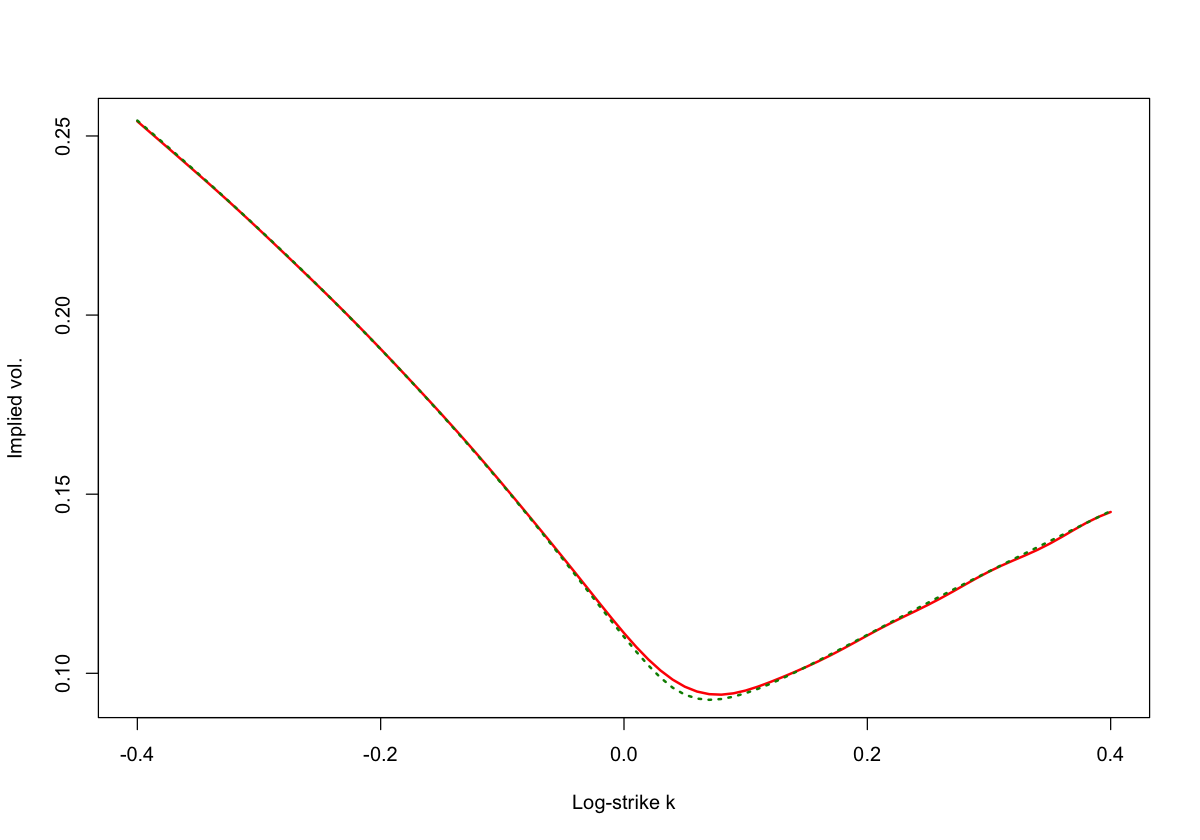
\includegraphics[width = \linewidth]{SmileComparison2}
%\caption{The red line is the Pad� approximation. The brown, blue, green and orange lines are from the QE simulation using 100,000 paths with 10, 200, 400, 1000 steps respectively.}
\caption{The red line is from the Adams scheme with 5,000 steps. The blue dashed line is from the QE simulation using 100,000 paths and 1,000 steps.
%; the blue dotted line is from the QE simulation using 10,000 paths and 5,000 steps.   
We see numerical evidence of convergence!}
\label{fig:SmileComparison}
\end{center}
\end{figure}



%%%%%%%%%%%%%%%%%%%%%%%%%%%%%%%%%%%%%%%%%%%%%%%
\section{A QE hybrid scheme}%: Third attempt}

The scheme \eqref{eq:Euler} matches means and variances at each step but it does not match the covariance structure of the process.  For example, consider the covariance 
between $v_1$ and $\hat \xi_2$ which from \eqref{eq:covariances} is given approximately by
 \beas
 \cov[v_1,\hat \xi_2] =   \bar \xi\,\cG_{0,1}(\Delta).
 \eeas
\eqref{eq:Euler} and \eqref{eq:xiHatEuler} approximate this covariance as
$
\cov[v_1,\hat \xi_2]  \approx \bar \xi\,b_2^\star\,b_1^\star\,\Delta
$
which is equivalent to the approximation
\beq
\left(\int_{0}^{\Delta}\,g(s)\, g( s+ \Delta )\,ds\right)^2 \approx 
\left( \int_{0 }^{ \Delta}\,g^2(s)\,ds\right)\,\left( \int_{0 }^{ \Delta}\,g^2(s+\Delta)\,ds\right), 
\label{eq:EulerApprox}
\eeq
which, though exact in the case of an exponential kernel, 
  is obviously inaccurate for small $H$.
The essence of the hybrid scheme with $\kappa=1$ of \cite{bennedsen2017hybrid} is to correct the error in the approximation \eqref{eq:EulerApprox} by simulating another random variable that is uncorrelated with changes in $v_k$ so as to match the covariance of $v_1$ and $v_2$.

One could add further corrections so as to correct (for example) the covariance of $v_1$ and $v_3$.  However, for small $H$ such higher order corrections are small and seem not to improve the performance of the algorithm\footnote{I conjecture that we can prove that higher order corrections are negligible for $H$ small.}.  This is as we would expect because the decay of the autocorrelation function is very fast for small $H$; we would only see the impact of higher order corrections if we were to choose very tiny time steps.


\subsection{ A 2-D version of the QE step}
Let
\beas
u_1 &=& \int_0^\Delta\,g(\Delta-s)\,\sqrt{v_s}\,dW_s\\
\chi_1 &=&  \int_0^\Delta\,\sqrt{v_s}\,dW_s.
\eeas
Linear regression gives
\beas
u_1 = \beta_{v\chi}\,\chi_1 + \epsilon_1
\eeas
where $\epsilon$ and $\chi$ are independent.  From \eqref{eq:covariances},
\beas
\beta_{v\chi}= \frac{\cG_{0,0}(\Delta)}{\Delta} = b_1^\star.
\eeas
Again from \eqref{eq:covariances}, we have
\beas
\var[u_1]&=& \bar \xi \,\cG_{0,0}(\Delta)\\
\var[\chi_1]&=& \bar \xi \,\Delta\\
\var[\epsilon_1] &=& \var[u_1]-\beta_{v\chi}^2\,\var[\chi_1] = \bar \xi \,\cG_{0,0}(\Delta)\,(1-\rho_{v\chi}^2). 
\eeas
Let's generate both $\chi_1$ and $\epsilon_1$ separately using the QE scheme.
%, for the sake of concreteness, with the same variance ratio $\psi$.  
In particular, since $v_1 \geq 0$, we must have
\[
 \beta\,\chi_1 + \epsilon_1 +\xi_1 \geq 0.
\]
Thus for some  $a>0$, we must have
\[
 \beta\,\chi_1 + a\,\xi_1 \geq 0;\quad  \epsilon_1 + (1-a)\,\xi_1\geq 0.
\]
That gives
\beas
\ee{ \beta\,\chi_1 + a\,\xi_1}^2 &=&a^2\,\xi_1^2= \psi_\chi\,\beta^2\,\bar \xi \,\Delta
=\psi_\chi\,\rho_{v\chi}^2\,\bar \xi \,\cG_{0.0}(\Delta) \\
\ee{ \epsilon_1 + (1-a)\,\xi_1}^2 &=& (1-a)^2\,\xi_1^2=\psi_\epsilon\, \bar \xi \,\cG_{0,0}(\Delta)\,(1-\rho_{v\chi}^2).
\eeas
Once again approximating $\bar \xi = \xi_1$, and solving for $a$, we find that there is a solution only when $a=\tfrac12$.  Thus we need to solve the system
\beas
\tfrac14 \xi_1^2&=& \psi_\chi\,\bar \xi \,\cG_{0,0}(\Delta)\,\rho_{v\chi}^2\\
\tfrac14 \xi_1^2&=&\psi_\epsilon\, \bar \xi\,(1-\rho_{v\chi}^2) \,\cG_{0,0}(\Delta).
\eeas
This gives
\bea
 \psi_\chi = \frac{ \bar \xi_1}{4\,\cG_{0,0}(\Delta)\,\rho_{v\chi}^2};\quad
 \psi_\epsilon = \frac{ \bar \xi_1}{4\,\cG_{0,0}(\Delta)\,(1-\rho_{v\chi}^2)}.
 \label{eq:psi2}
\eea


\noindent We have now, at least in principle, generated the non-negative random variables $\chi_1$ and $\epsilon_1$ and so we also have $v_1=\xi_1+\beta_{v\chi}\,u_1 + \epsilon_1$.  

\subsubsection{A first small $H$ approximation}

According to the approximate covariance matrix \eqref{eq:Rapprox}, $\hat \xi_2$ is perfectly correlated with $\chi_1$.  
Moreover $\ee{\chi_1}=0 $ so we may write
\beq
 \hat \xi_2-\xi_2 \approx \frac{\sqrt{\var[\hat \xi_2]}}{\sqrt{\var[\chi_1]}}\,\chi_1\\
\approx \sqrt{\frac{\cG_{1,1}(\Delta)}{\Delta}}\chi_1 =b_2^\star\,\chi_1.
\label{eq:chi1}
\eeq

\red{
\begin{remark}
We can come back and generalize this step later. But we expect the correction to be very small.
\end{remark}
}

\subsection{The generic step}

Recall that in the Euler-style case,
\beas
v^E_n = \xi_n + \sum_{k=1}^{n}\,b^\star_{n-k+1}\,\chi_k.
\eeas
In analogy with \cite{bennedsen2017hybrid}, we write our proposed hybrid scheme as
\beas
v^H_n = \xi_n + u_n + \sum_{k=1}^{n-1}\,b^\star_{n-k+1}\,\chi_k,
\eeas
where $u_n$ is no longer approximated as $b_1^\star\,\chi_n$.
Thus for $n>1$,  given $\cF_{n-1}$, dropping the superscript $H$ for ease of notation, generate $\chi_n$ and $\epsilon_n$ together using the 2-D QE scheme with
\beas
\ee{\beta\,\chi_n|\cF_{n-1}}&=\tfrac12 \hat \xi_{n}; \quad \ee{\epsilon_n|\cF_{n-1}}&=\tfrac12 \hat \xi_{n}; \\
\var[\chi_n|\cF_{n-1}]&=\bar \xi_n\, \Delta;\quad  \var[\epsilon_n|\cF_{n-1}]&=\bar \xi\,\cG_{0,0}(\Delta),
\eeas
and 
\[
\bar \xi_n =  \frac{1}{2 H + 1}\, \left[\hat \xi_n +  2 H\,v_{n-1}\right].
\]
Then with\footnote{Look at $b^\star$ as the root mean square average of $g$ to see the expression for $b^\star$.}
\[
 \beta= \frac{\cG_{0,1}(\Delta)}{\cG_{0,0}(\Delta)};\quad 
 \rho =\frac{\cG_{0,1}(\Delta)}{ \sqrt{\cG_{0,0}(\Delta)}\sqrt{\cG_{1,1}(\Delta)}};
 \quad b^\star_j = \sqrt{\frac{\cG_{0,0}(j \Delta)-\cG_{0,0}((j-1)\Delta)}{\Delta}},
\]
compute $\hat \xi_{n+1}$ as
\beq
\hat \xi_{n+1} =  \xi_{n+1} +  \sum_{k=1}^{n}\,b^\star_{n-k+1}\,\chi_k.
\label{eq:xihatUpdate}
\eeq
\begin{remark}
After implementing \eqref{eq:xihatUpdate}, it seems that $\hat \xi_{n+1} > 0$.  Maybe we can prove this?
\end{remark}

%\subsubsection{Check of terminal variance}

\subsection{Numerical results}

In Figure \ref{fig:SmileComparison3} we compare 1-year smiles generated with the above hybrid QE scheme with those generated using the Euler-like scheme of Section \ref{sec:Euler} and using the Adams scheme with 5,000 steps.  Again, the parameters used were:
$$
\xi(u) = 0.025;\, H = 0.05;\, \nu = 0.4; \rho=-0.65.
$$
Note that $\nu$ in the original formulation of the rough Heston model and $\eta$ in \eqref{eq:GammaKernel}
are related as
$$
\eta = \frac{\nu}{\sqrt{2 H}\, \Gamma(\alpha)}.
$$

\begin{figure}[htbp]
\begin{center}
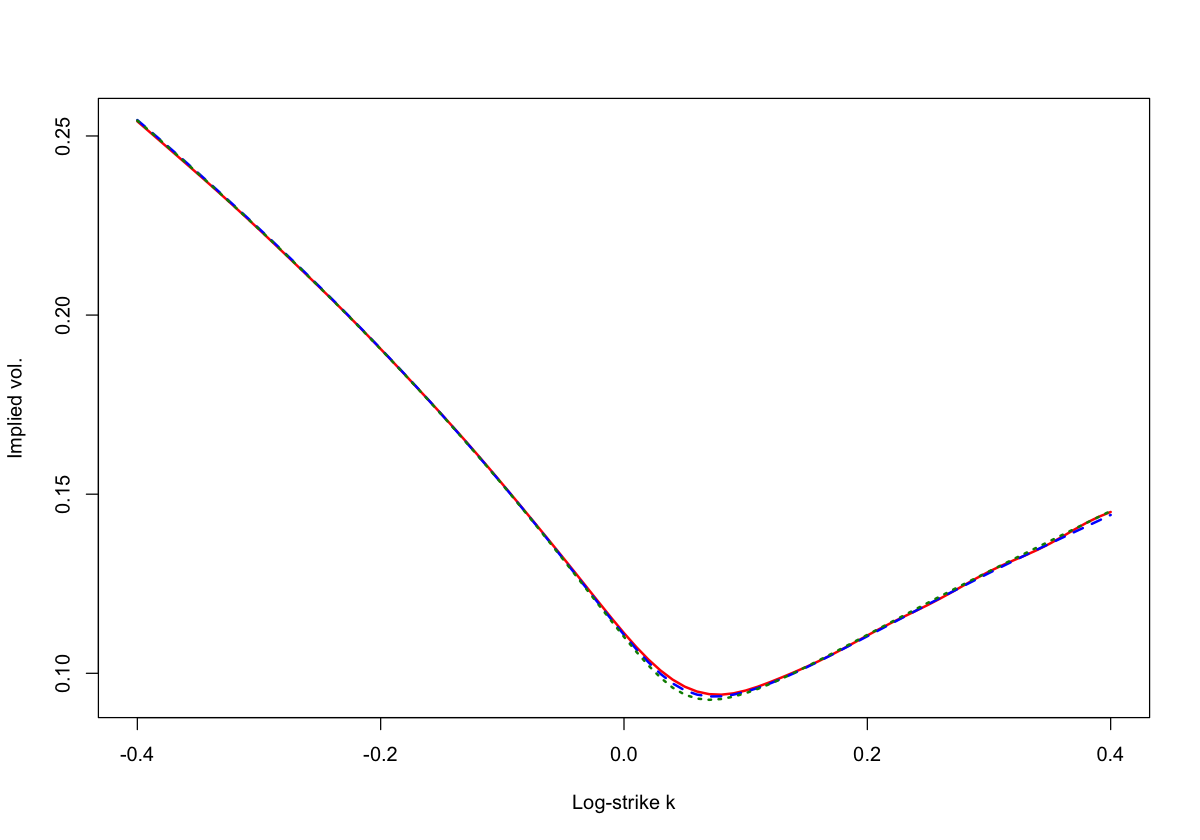
\includegraphics[width = \linewidth]{SmileComparison3}
%\caption{The red line is the Pad� approximation. The brown, blue, green and orange lines are from the QE simulation using 100,000 paths with 10, 200, 400, 1000 steps respectively.}
\caption{The red line is from the Adams scheme with 5,000 steps. The blue dashed line is from the hybrid QE simulation using 100,000 paths and 1,000 steps; the green dotted line is from the Euler QE simulation with 100,000 paths and 1,000 steps.
%; the blue dotted line is from the QE simulation using 10,000 paths and 5,000 steps.   
We see that the hybrid scheme is marginally but significantly better.}
\label{fig:SmileComparison3}
\end{center}
\end{figure}

In Figure \ref{fig:SmileComparison200}, we see that 200 steps using the hybrid scheme seems to be a good compromise between speed and accuracy.  Note that a back-of-the-envelope estimate says that a 200 step computation should run approximately 25 times faster than a 1,000 step one.


\begin{figure}[htbp]
\begin{center}
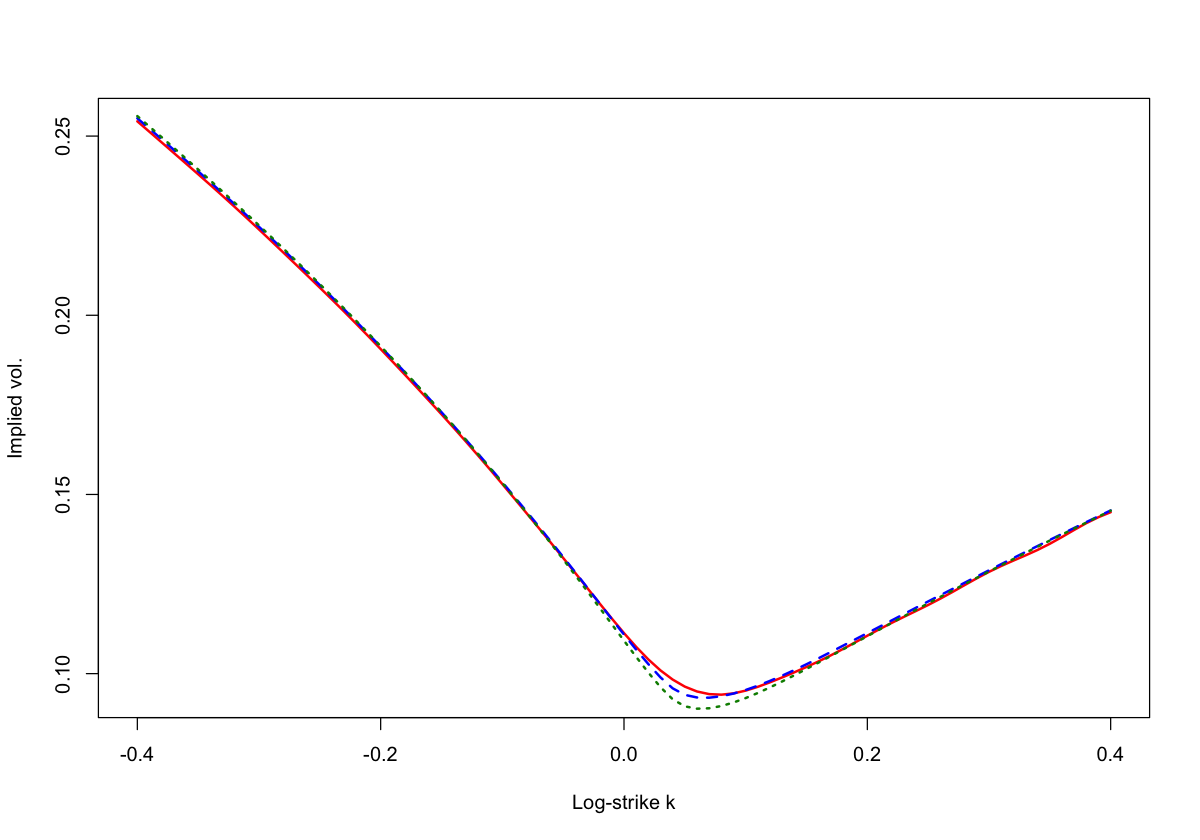
\includegraphics[width = \linewidth]{SmileComparison200}
%\caption{The red line is the Pad� approximation. The brown, blue, green and orange lines are from the QE simulation using 100,000 paths with 10, 200, 400, 1000 steps respectively.}
\caption{The red line is from the Adams scheme with 5,000 steps. The blue dashed line is from the hybrid QE simulation using 100,000 paths and 200 steps; the green dotted line is from the Euler QE simulation with 100,000 paths and 200 steps.
%; the blue dotted line is from the QE simulation using 10,000 paths and 5,000 steps.   
We see that the hybrid scheme is marginally but significantly better.}
\label{fig:SmileComparison200}
\end{center}
\end{figure}


\subsection{Probabilistic interpretation of the hybrid scheme}

The Euler scheme can be seen as simulation of the rough process as if it were a semimartingale.  The hybrid scheme (with $\kappa=1$) adds independent noise at each step.  In some sense the hybrid scheme represents the rough process as a semimartingale plus independent noise.  Indeed, that a semimartingale sampled with (independent) measurement error may look rough has been noticed before, see the detailed discussion in \cite{fukasawa2019volatility}. 
% It takes extra work to distinguish between independent noise and true roughness.

In the limit of many components, the Markovian approximation of \cite{abijaber2018multifactor} corresponds to the Euler scheme \eqref{eq:Euler}.  As pointed out in that paper, the simulated process is a semimartingale that scales as a rough process as the sampling interval increases.  Adding the independent noise $Z^\perp$ as each step restores apparent roughness for every sampling interval.

%\begin{remark}
%Intuitively, in order to get a good simulation of $y$ and therefore of $v$, we need to include the orthogonal component at each step.
%\end{remark}

\subsection{Financial interpretation of the hybrid scheme}

Since $v_0=\xi_0(0)$ is given, the first step is almost exact.
\[
v_1 = \xi_1 + \eta\,\sqrt{w(\Delta)}\,\sqrt{v_0}\,Z_1 .
\]
The next step is
\beas
v_2 &=& \xi_2 + \int_0^{2 \Delta}\,g(2 \Delta-s)\,\sqrt{v_s}\,dW_s\\
&=& \xi(2 \Delta) +\int_0^{\Delta}\,g(2 \Delta-s)\,\sqrt{v_s}\,dW_s
+ \int_{\Delta}^{2 \Delta}\,g(2 \Delta-s)\,\sqrt{v_s}\,dW_s\\
&\approx& \left\{\xi_2 +\sqrt{v_0}\,\int_0^{\Delta}\,g(2 \Delta-s)\,dW_s \right\}
+ \sqrt{v_1}\,\int_{0}^{\Delta}\,g(s)\,dW_s.
\eeas
The term in brackets, represent the forward variance curve after one simulation step.  That is
\[
\eets{v_2}{\Delta}= \xi_2 +\sqrt{v_0}\,\int_0^{\Delta}\,g(2 \Delta-s)\,dW_s.
\]
The hybrid correction term $v^{corr}$ in \eqref{eq:hybridCorr} corresponds to computing the expectation of 
\[
\int_0^{\Delta}\,g(2 \Delta-s)\,\sqrt{v_s}\,dW_s
\]
conditional on $\int_0^{\Delta}\,g( \Delta-s)\,dW_s$ by linear regression.  Generalizing this argument, we may rewrite the hybrid scheme \eqref{eq:hybrid} as
\bea
v^H_n &=& \hat \xi_{n} +  \sqrt{v_{n-1}}\,b^\star_{1}\,\sqrt{\Delta}\,\left(\rho_1 Z_n + \bar \rho_1 Z_n^\perp \right)
\label{eq:hybrid2}
\eea
with
\beas
\hat \xi_{n} :=  \eets{v_n}{(n-1)\Delta}=\xi_n + \sum_{k=1}^{n-1}\,\sqrt{v_{k-1}}\,b^\star_{n-k+1}\,\sqrt{\Delta}\,Z_k.
\eeas
In words, at time $(n-1)\Delta$, add a martingale increment to the expectation of $v_n$ given $\cF_{(n-1)\Delta}$.   We see explicitly that $\eets{v_n}{(n-1)\Delta}$ takes into account the whole history of the increments $Z_k, k <n$.

\section{Numerical tests of convergence}

After extensive testing, it appears that the order of weak convergence of the hybrid scheme is one.  That being the case, we may assume that the exact smile is given by Richardson extrapolation of the smiles computed with 1,000 and 500 time steps respectively.  This allows estimation of the bias of the hybrid scheme as a function of the number of time steps.  In Figure \ref{fig:convergence}, we plot smiles with various numbers of time steps and plot errors vs time steps. Order one weak convergence is clearly demonstrated.

\begin{figure}[htbp]
\begin{center}
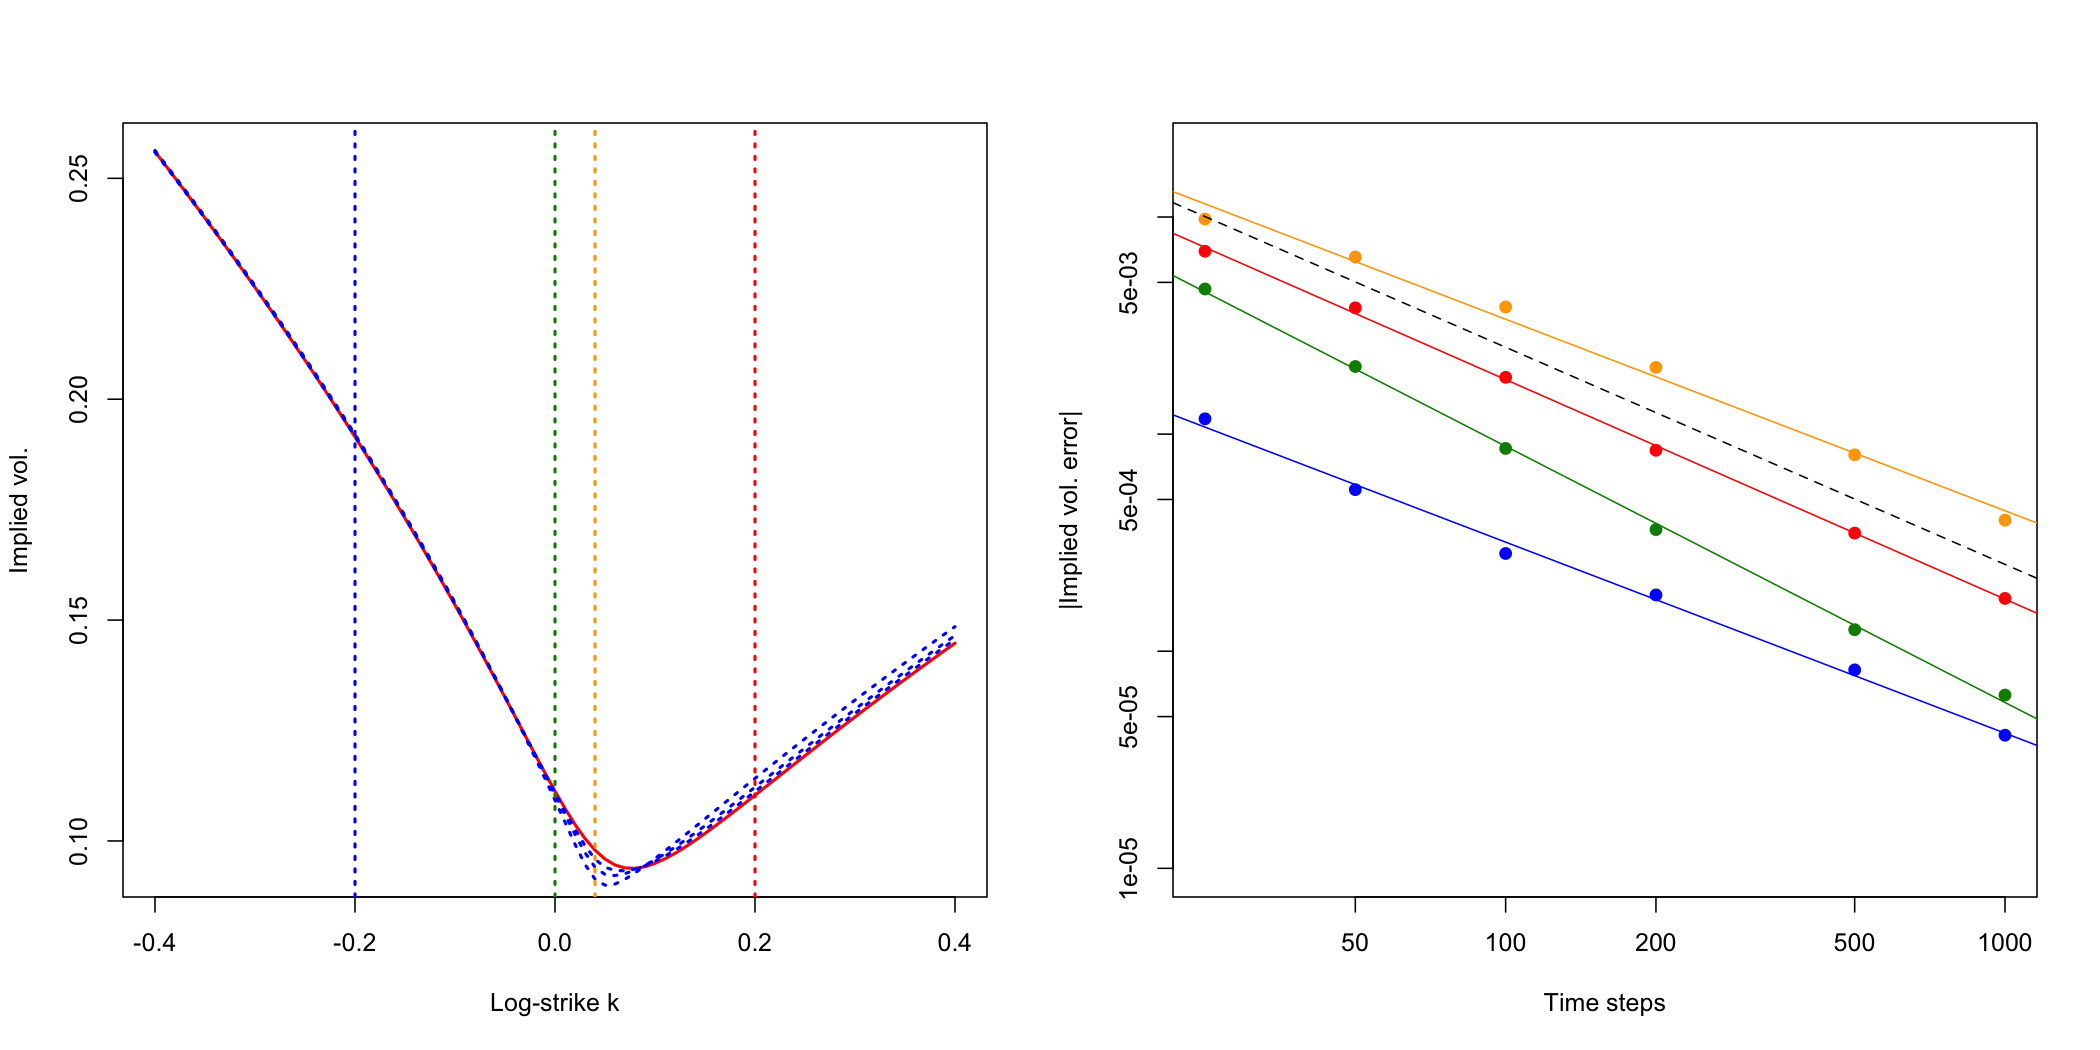
\includegraphics[width = \linewidth]{convergence}

\caption{In the LH plot, the red line is from Richardson extrapolation of 1,000 and 500 time steps smiles. The blue dotted lines are smiles computed with various lower numbers of time steps.  In the RH plot, we plot absolute implied volatility errors vs time steps, for various log-strikes: $k \in \{-0.2,0,04,0.2\}$ with colors corresponding to the vertical lines in the LH plot.  The dashed black line with slope $-1$ is plotted for reference, clearly demonstrating order one weak convergence.  All simulations are with 10 million time steps.}\label{fig:convergence}
\end{center}
\end{figure}

\subsection{Richardson extrapolation}

Given the apparent order one weak convergence of the hybrid scheme, we may compute various Richardson extrapolated smiles and plot their estimated errors.  We plot results in Figure \ref{fig:convergenceRichardson}.

\begin{figure}[htbp]
\begin{center}
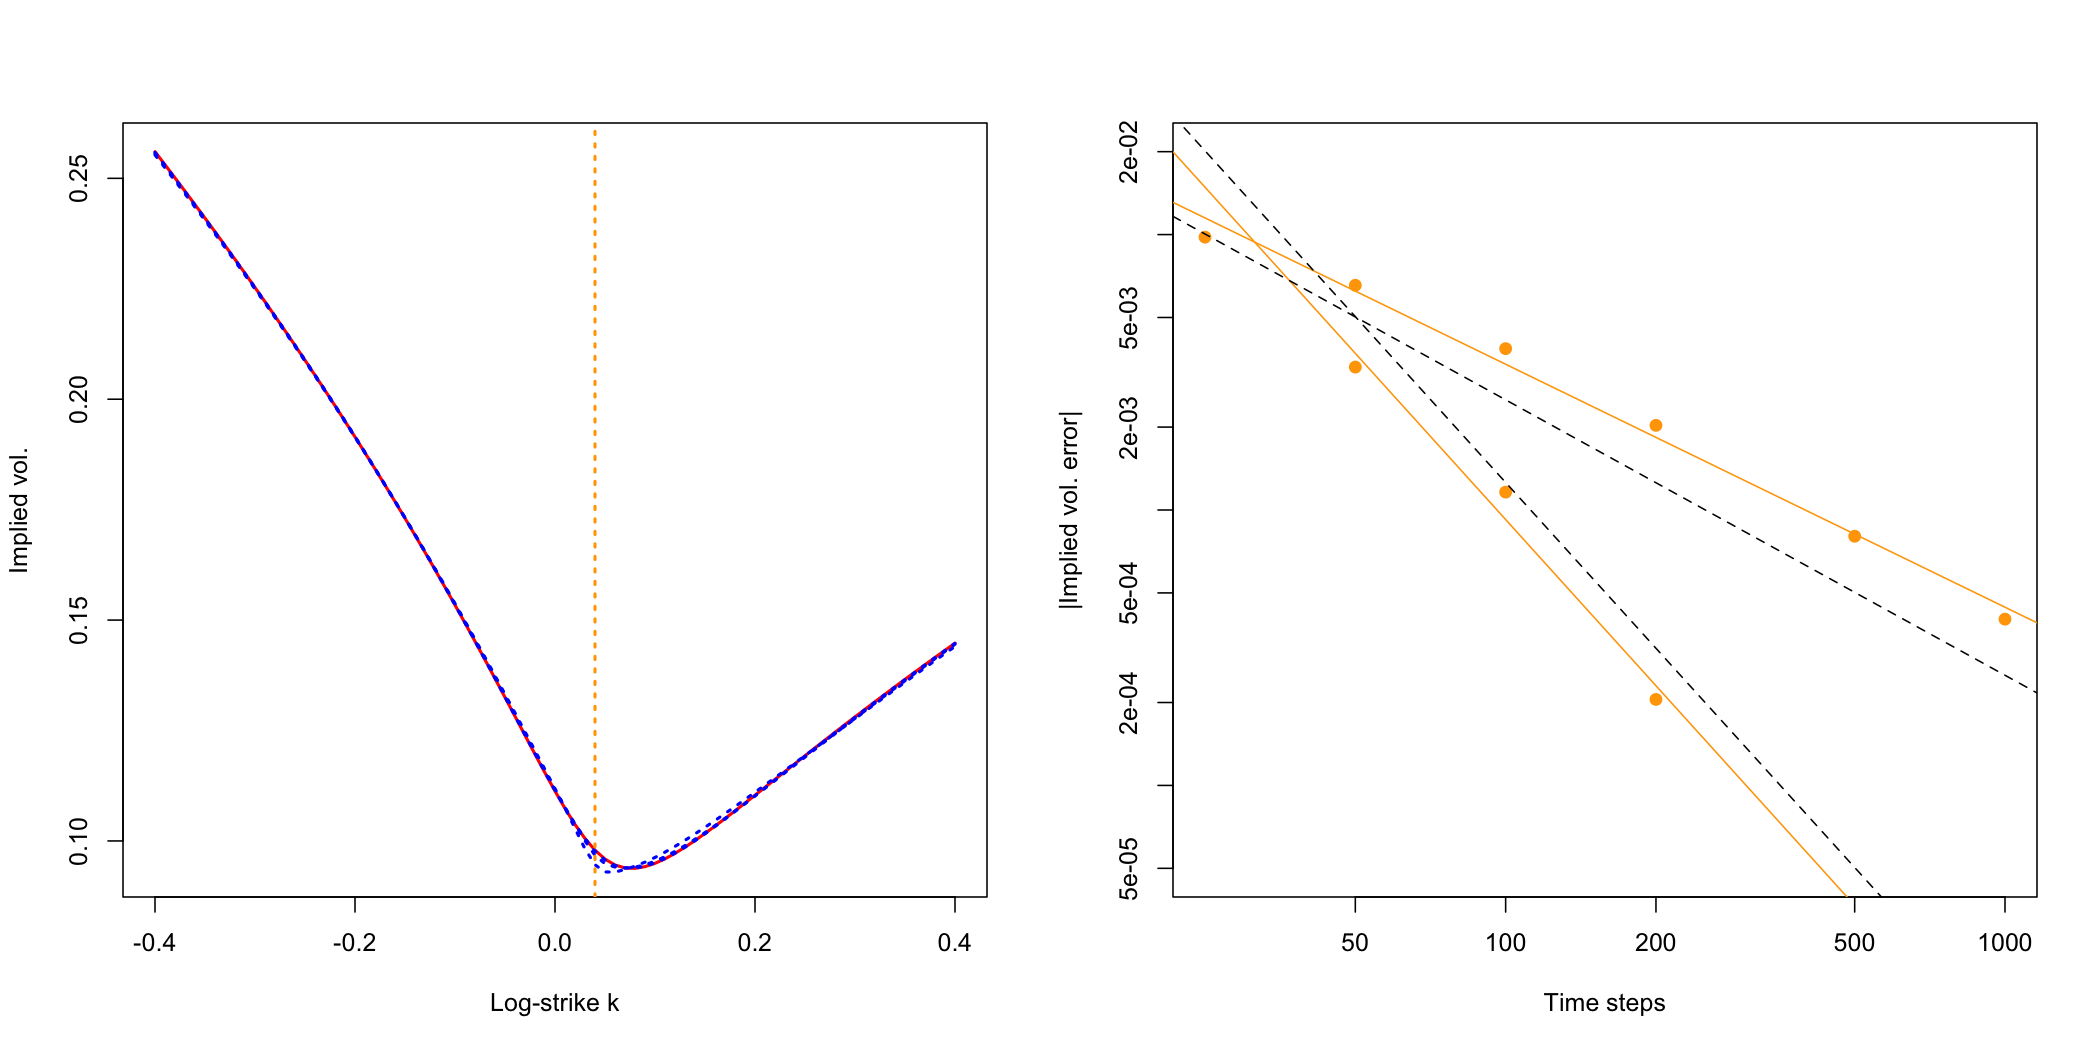
\includegraphics[width = \linewidth]{convergenceRichardson}

\caption{In the LH plot, the red line is from Richardson extrapolation of 1,000 and 500 time steps smiles. The blue dotted lines are smiles computed using Richardson extrapolation with various lower numbers of time steps.  In the RH plot, we plot absolute implied volatility errors vs time steps, for log-strike $k=0.04$, the orange vertical line in the LH plot, where errors are maximized.  Errors without extrapolation are superimposed for reference as are black-dashed lines with slopes $-1$ and $-2$ respectively.  We see evidence of order 2 weak convergence of Richardson-extrapolated smiles.  All simulations are with 10 million time steps.}
\label{fig:convergenceRichardson}
\end{center}
\end{figure}

%\begin{figure}[htbp]
%\begin{center}
%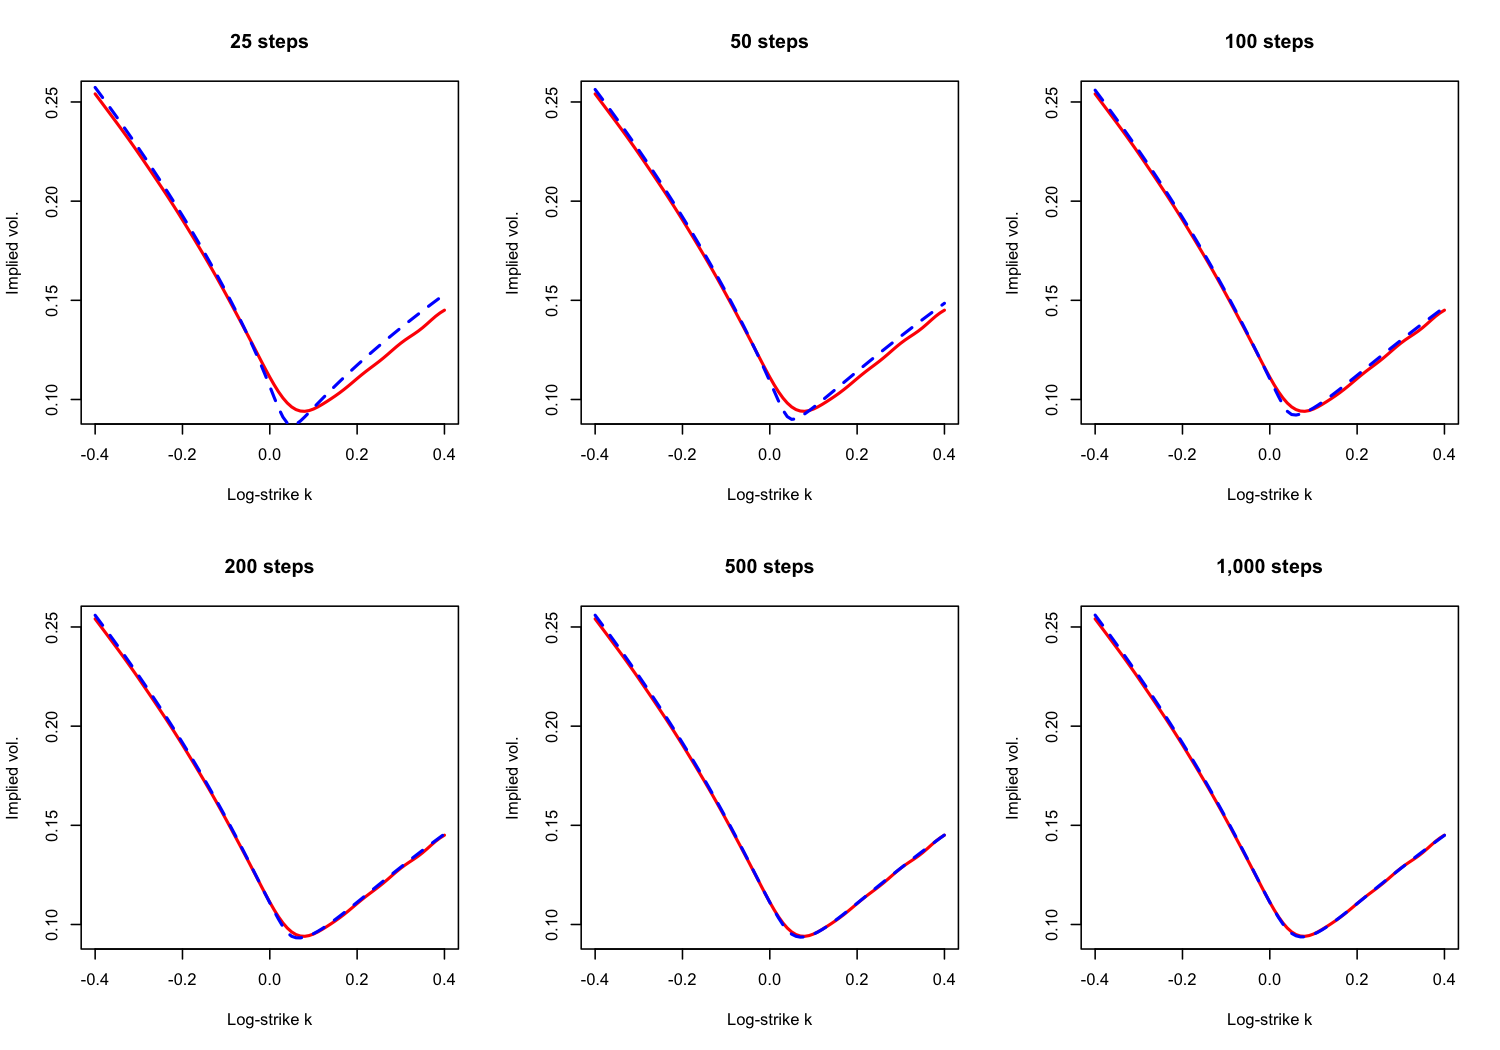
\includegraphics[width = \linewidth]{HybridSmiles}
%%\caption{The red line is the Pad� approximation. The brown, blue, green and orange lines are from the QE simulation using 100,000 paths with 10, 200, 400, 1000 steps respectively.}
%\caption{The red line is from the Adams scheme with 5,000 steps. The blue dashed line is from the hybrid QE simulation using 100,000 paths and 200 steps; the green dotted line is from the Euler QE simulation with 100,000 paths and 200 steps.
%%; the blue dotted line is from the QE simulation using 10,000 paths and 5,000 steps.   
%We see that the hybrid scheme is marginally but significantly better.}
%\label{fig:SmileComparison200}
%\end{center}
%\end{figure}



\bibliographystyle{alpha}
\bibliography{RoughVolatility}

\begin{appendix}

\section{Approximate variance}

For a kernel $g$ that is the product of a power-law and a regularly varying function, we have the following very natural-looking approximation of the variance over a timestep.
\begin{lemma}\label{lem:varvApprox}
Let 
\[
\cG_{0,0}(\Delta)=\int_0^\Delta\,g(s)^2\,ds. 
\]
Then
\beq
\var[v_\Delta]\approx \frac{\cG_{0,0}(\Delta)}{2 H + 1}\, \left[\xi(\Delta) +  2 H\,v_0\right].
\label{eq:varv}
\eeq
\end{lemma}

\begin{proof}

We approximate the variance after one step as follows.
\beas
\var\left[v_\Delta\right] &=& \int_0^\Delta\,\xi(s)\,g(\Delta-s)^2\,ds\\
&=& \xi(\Delta)\,\int_0^\Delta\,g(\Delta-s)^2\,ds -  \int_0^\Delta\,\xi'(s)\,ds\,\int_0^s\,g(\Delta-r)^2\,dr\\
&\approx & \xi(\Delta)\,\int_0^\Delta\,g(s)^2\,ds  -  \left[\xi(\Delta)-v_0\right]\,\frac1 \Delta\,\int_0^\Delta\,ds\int_0^s\,g(\Delta-r)^2\,dr\\
&= & \xi(\Delta)\,\int_0^\Delta\,g(s)^2\,ds  -  \left[\xi(\Delta)-v_0\right]\,\frac1 \Delta\,\int_0^\Delta\,g(s)^2\,s\,ds.
\eeas
Now let
$
g(\tau)=\tau^{H-1/2}\,L_g(\tau),\, \tau\in(0,T]
$.
Then, for some $s^\star \in [0,T]$,
\beas
\var\left[v_\Delta\right] &\approx & \xi(\Delta)\,L_g(s^\star)^2\,\frac{\Delta^{2 H}}{2 H}   -  \left[\xi(\Delta)-v_0\right]\,\,L_g(s^\star)^2\,\frac{\Delta^{2 H}}{2H +1}.
\eeas
Also
\[
L_g(s^\star)^2\,\frac{\Delta^{2 H}}{2 H} \approx \int_0^\Delta\,g(s)^2\,ds = \cG_{0,0}(\Delta),
\]
which completes the proof.
\end{proof}
\begin{remark}
Note that in the limit $H \to 0$, all of the weight is on the end of the interval.
\end{remark}

\begin{remark}\label{rmk:error}

From the above proof, we see that given sufficient smoothness of $\xi$,
$$
\var\left[v_\Delta\right] =  \frac{\cG_{0,0}(\Delta)}{2 H + 1}\, \left[\xi(\Delta) +  2 H\,v_0\right] +\cO(\Delta^{2 H + 1}).
$$
\end{remark}

\noindent Similarly, we have the following lemma.
\begin{lemma}\label{lem:covyApprox}
Let
\beas
v_\Delta = \xi + \int_0^\Delta\,g(\Delta-s)\,\sqrt{v_s}\,dW_s, \quad
\chi_\Delta = \int_0^\Delta\,\sqrt{v_s}\,dW_s.
\eeas
Further let 
\[
\cG_0(\Delta)=\int_0^\Delta\,g(s)\,ds. 
\]
Then
\beq
\cov[v_\Delta,\chi_\Delta]\approx \frac{\cG_0(\Delta)}{\alpha+1}\, \left[\xi(\Delta) +  \alpha\,v_0\right].
\label{eq:varv}
\eeq
\end{lemma}

\begin{proof}

We approximate this covariance after one step as follows.
\beas
\cov[v_\Delta,Y_\Delta] &\approx& \int_0^\Delta\,\xi(s)\,g(\Delta-s)\,ds\\
&=& \xi(\Delta)\,\int_0^\Delta\,g(\Delta-s)\,ds -  \int_0^\Delta\,\xi'(s)\,ds\,\int_0^s\,g(\Delta-r)\,dr\\
&\approx & \xi(\Delta)\,\int_0^\Delta\,g(s)\,ds  -  \left[\xi(\Delta)-v_0\right]\,\frac1 \Delta\,\int_0^\Delta\,ds\int_0^s\,g(\Delta-r)\,dr\\
&= & \xi(\Delta)\,\int_0^\Delta\,g(s)\,ds  -  \left[\xi(\Delta)-v_0\right]\,\frac1 \Delta\,\int_0^\Delta\,g(s)\,s\,ds.
\eeas
Now let
$
g(\tau)=\tau^{H-1/2}\,L_g(\tau),\, \tau\in(0,T]
$.
Then, for some $s^\star \in [0,T]$,
\beas
\cov[v_\Delta,Y_\Delta] &\approx & \xi(\Delta)\,L_g(s^\star)\,\frac{\Delta^{\alpha}}{\alpha}   -  \left[\xi(\Delta)-v_0\right]\,\,L_g(s^\star)\,\frac{\Delta^{\alpha}}{\alpha +1}.
\eeas
Also
\[
L_g(s^\star)\,\frac{\Delta^{\alpha}}{\alpha} \approx \int_0^\Delta\,g(s)\,ds = \cG_0(\Delta),
\]
which completes the proof.
\end{proof}

\section{Bell polynomials}

$$
B_{n,k}(x_1,x_2,\dots,x_{n-k+1}) = \sum{n! \over j_1!j_2!\cdots j_{n-k+1}!}
\left({x_1\over 1!}\right)^{j_1}\left({x_2\over 2!}\right)^{j_2}\cdots\left({x_{n-k+1} \over (n-k+1)!}\right)^{j_{n-k+1}},
$$
where the sum is taken over all sequences $j_1,j_2,j_3,...,J_{n-k+1}$ of non-negative integers such that these two conditions are satisfied:
\beas
j_1 + j_2 + \cdots + j_{n-k+1} &=& k,\\
j_1 + 2 j_2 + 3 j_3 + \cdots + (n-k+1)j_{n-k+1} &=& n.
\eeas
The sum
$$
B_n(x_1,\dots,x_n)=\sum_{k=1}^n B_{n,k}(x_1,x_2,\dots,x_{n-k+1})
$$
is called the $n$th ``complete exponential Bell polynomial".



\end{appendix}

\end{document}





%%% Local Variables:
%%% mode: latex
%%% TeX-master: t
%%% End:
